%% =========================================================================
%% Springer Nature LaTeX Template for Neural Computing and Applications (NCAA)
%% Document Class: sn-jnl with sn-mathphys-num
%% Author: Phu Toan Nguyen
%% Affiliation: Faculty of Information Technology, Hanoi University of Business and Technology (HUBT), Hanoi, Vietnam
%% =========================================================================

\documentclass[pdflatex,sn-mathphys-num,referee,lineno]{sn-jnl}

%% --- Mathematics Packages ---
\usepackage{amsmath}
\usepackage{amssymb}
\usepackage{amsfonts}
\usepackage{amsthm}
\usepackage{bm}              % Bold math symbols (\bm{\theta}, \bm{\mu})
\usepackage{mathtools}       % Advanced math enhancements

%% --- Professional Tables (Strict Springer Table Standards) ---
\usepackage{booktabs}        % Mandatory (\toprule, \midrule, \botrule)
\usepackage{multirow}        % Multi-row table cells
\usepackage{tabularx}        % Auto-sizing table columns
\usepackage{makecell}        % Multi-line header cells

%% --- Graphics and Floats ---
\usepackage{graphicx}        % Inclusion of EPS/PNG/PDF figures
\usepackage{subcaption}      % Subfigures ((a), (b), (c))
\usepackage{float}           % Float placement controls

%% --- Algorithms ---
\usepackage{algorithm}       % Algorithm float wrapper
\usepackage{algpseudocode}   % Algorithmic pseudocode styling

%% --- Hyperlinks and Metadata ---
\usepackage{url}
\usepackage{hyperref}
\hypersetup{
    colorlinks=true,
    linkcolor=blue,
    citecolor=blue,
    filecolor=magenta,      
    urlcolor=cyan,
    pdftitle={PSO-TCWavKAN: Power Transformer Thermal Dynamics Forecasting},
    pdfauthor={Phu Toan Nguyen}
}

%% --- Theorem Environments (Standard Springer Nature Hooks) ---
\theoremstyle{thmstyleone}
\newtheorem{theorem}{Theorem}[section]
\newtheorem{proposition}[theorem]{Proposition}
\newtheorem{lemma}[theorem]{Lemma}
\newtheorem{corollary}[theorem]{Corollary}

\theoremstyle{thmstyletwo}
\newtheorem{example}{Example}[section]
\newtheorem{remark}{Remark}[section]

\theoremstyle{thmstylethree}
\newtheorem{definition}{Definition}[section]

\raggedbottom

\begin{document}

\title[PSO-TCWavKAN for Transformer Thermal Dynamics]{PSO-TCWavKAN: Swarm-Optimized Temporal Continuous Wavelet Kolmogorov–Arnold Networks for Power Transformer Thermal Dynamics Forecasting}

\author*[1]{\fnm{Phu Toan} \sur{Nguyen}}\email{nphu211206@gmail.com}

\affil*[1]{\orgdiv{Faculty of Information Technology}, \orgname{Hanoi University of Business and Technology (HUBT)}, \orgaddress{\street{No. 29A, Lane 124, Vinh Tuy Street, Vinh Hung Ward, Hai Ba Trung District}, \city{Hanoi}, \postcode{100000}, \country{Vietnam}}}

\abstract{Power transformer thermal dynamics forecasting is vital for assessing insulation degradation, preventing catastrophic dielectric breakdown, and enabling Dynamic Thermal Rating in modern smart grids. In accordance with IEEE Std C57.91-2011, top-oil and winding temperatures directly dictate asset loss-of-life via the Arrhenius model. However, existing Long-Term Time Series Forecasting (LTSF) paradigms face significant structural bottlenecks: self-attention Transformers exhibit quadratic complexity $\mathcal{O}(L^2)$ and temporal permutation vulnerabilities, linear baselines underfit multi-frequency thermal inertia, and standard Kolmogorov–Arnold Networks (KAN) suffer from discrete B-spline grid instability during continuous distribution shift. To overcome these limitations, this paper proposes PSO-TCWavKAN, a unified hybrid deep learning framework. Our architecture integrates Invertible Reversible Instance Normalization (RevIN) with detached statistics, a dual-branch depthwise temporal convolution module, and continuous Morlet wavelet KAN layers featuring smooth analytic gradients across the entire real domain. To circumvent sub-optimal local minima in the multi-scale wavelet parameter landscape, we deploy a Comprehensive Learning Particle Swarm Optimizer (CLPSO) governed by Clerc's constriction factor ($\chi = 0.72984$) on a leak-free surrogate proxy. We formally prove that PSO-TCWavKAN achieves strictly linear computational complexity $\mathcal{O}(DN)$. Evaluated across 16 canonical configurations on ETTh1 and ETTh2 telemetry, PSO-TCWavKAN delivers an average 12.30\% MSE reduction over DLinear, confirmed statistically significant by the Wilcoxon signed-rank test ($p = 3.05 \times 10^{-5}$).}

\keywords{Kolmogorov–Arnold Networks (KAN), Continuous Wavelet Transform, Particle Swarm Optimization, Power Transformer Thermal Dynamics, Reversible Instance Normalization, Long-Term Time Series Forecasting}

\maketitle

%% =========================================================================
%% SECTION 1: INTRODUCTION
%% =========================================================================
\section{Introduction}\label{sec:introduction}

\subsection{Physical Stakes of Transformer Thermal Dynamics}\label{subsec:physical_stakes}
Power transformers represent critical capital assets in modern electrical transmission and distribution grids, whose operational reliability and asset longevity fundamentally govern broad system resilience \cite{alvarez2019transformer, tang2004simplified}. Within oil-immersed power transformers, operational lifespan is dictated almost exclusively by the progressive thermodynamic and chemical degradation of cellulose paper insulation surrounding copper winding conductors \cite{susa2005dynamic, pradhan2004remaininglife}. In accordance with the IEEE Guide for Loading Mineral-Oil-Immersed Transformers (IEEE Std C57.91-2011) \cite{ieee2012c5791} and international standards IEC 60076-7 \cite{iec2018600767}, the thermal state of the transformer is characterized by two vital state variables: the top-oil temperature (TOT) and the winding hottest-spot temperature (HST). 

Under the physical Arrhenius reaction rate theory established by Montsinger \cite{montsinger1930loading} and formalized in IEEE Std C57.91-2011 \cite{arrhenius1889geschwindigkeit, ieee2012c5791}, the relative rate of insulation aging $V$ is governed by an exponential thermodynamic relationship:
\begin{equation}
V = \exp \left( \frac{E_A}{R \cdot (T_{\text{ref}} + 273.15)} - \frac{E_A}{R \cdot (\Theta_{\text{HST}} + 273.15)} \right),
\label{eq:arrhenius_aging}
\end{equation}
where $E_A$ is the activation energy of cellulose degradation ($E_A \approx 111\,\text{kJ/mol}$), $R = 8.314\,\text{J/(mol}\cdot\text{K)}$ denotes the universal gas constant, $T_{\text{ref}} = 110^{\circ}\text{C}$ is the standardized rated hot-spot reference temperature, and $\Theta_{\text{HST}}$ is the instantaneous hottest-spot temperature in degrees Celsius. Because of this exponential dependency, persistent operating thermal excursions of merely $6^{\circ}\text{C}$ to $10^{\circ}\text{C}$ above rated thresholds double the cellulose degradation rate, precipitating accelerated mechanical embrittlement of insulating paper, dielectric breakdown of insulating oil, and catastrophic transformer failure \cite{radakovic2003hotspot, swift2001fundamental}. 

Consequently, high-precision forecasting of top-oil thermal trajectories across extended horizons ($H \in [96, 720]$ hours) is imperative for transmission system operators. Accurate multi-step thermal prognostics unlocks Dynamic Thermal Rating (DTR) \cite{alvarez2019transformer}, enabling grid dispatchers to safely exploit available transmission transfer capacity during peak load periods without violating thermal risk boundaries or compromising asset health.

\subsection{Critique of Existing Long-Term Time Series Forecasting Paradigms}\label{subsec:critique_ltsf}
In recent years, Long-Term Time Series Forecasting (LTSF) has been predominantly driven by deep neural network architectures \cite{zhou2021informer, wu2021autoformer, zhou2022fedformer, nie2023patchtst, liu2024itransformer}. Despite substantial advances, existing LTSF paradigms exhibit structural deficiencies when applied to multi-horizon industrial telemetry:

\begin{enumerate}
    \item \textbf{Quadratic Attention Overhead and Temporal Invariance}: Canonical Transformer models utilizing self-attention mechanisms \cite{vaswani2017attention, zhou2021informer, wu2021autoformer} exhibit computational complexity and memory allocations that scale quadratically ($\mathcal{O}(L^2)$) with the lookback window length $L$. While efficient variants such as Reformer \cite{kitaev2020reformer}, Linformer \cite{wang2020linformer}, and FEDformer \cite{zhou2022fedformer} mitigate this overhead to $\mathcal{O}(L)$ or $\mathcal{O}(L \log L)$, self-attention mechanisms inherently possess temporal permutation invariance. As rigorously demonstrated by Zeng et al. \cite{zeng2023dlinear}, scrambling temporal token positions in standard Transformers yields marginal degradation on benchmark prediction errors, indicating that global dot-product attention frequently fails to preserve fine-grained localized temporal causality and phase progression in physical time series.
    \item \textbf{Underfitting in Linear Baselines}: To overcome Transformer over-parameterization, embarrassingly simple linear mapping networks—most notably DLinear and NLinear \cite{zeng2023dlinear}—were proposed. Although DLinear demonstrates remarkable efficiency and competitive accuracy on quasi-linear trends, its strictly linear mapping layers ($\mathbf{W} \in \mathbb{R}^{H \times L}$) lack representational capacity to capture complex non-linear thermodynamic interactions, such as buoyancy-driven fluid convective oil circulation and non-linear ambient meteorological forcing \cite{susa2005dynamic, gouda2021topoil}.
    \item \textbf{Distribution Drift and Scale Distortion}: Real-world transformer loading exhibits non-stationary distribution drift across seasonal cycles and volatile industrial loads. While Reversible Instance Normalization (RevIN) \cite{kim2022revin} was introduced to neutralize shift, standard implementations suffer from gradient contamination through normalization statistics and risk denominator instability during inverse affine mapping under quiescent loading.
\end{enumerate}

\subsection{The KAN Opportunity and the Discrete B-Spline Grid Update Dilemma}\label{subsec:kan_dilemma}
As an alternative to traditional Multi-Layer Perceptrons (MLPs), Kolmogorov–Arnold Networks (KAN) have recently emerged following the foundational formulations of Kolmogorov \cite{kolmogorov1957representation} and Arnold \cite{arnold1957representation}, revived in modern machine learning by Liu et al. \cite{liu2024kan}. Rather than placing fixed non-linear activation functions on nodes with linear edge weights, KANs position learnable univariate non-linear activation functions directly on network edges:
\begin{equation}
f(\mathbf{x}) = \sum_{q=1}^{2n+1} \Phi_q \left( \sum_{p=1}^n \phi_{q,p}(x_p) \right).
\label{eq:kan_foundational}
\end{equation}
In canonical KAN implementations \cite{liu2024kan}, the univariate edge activations $\phi(x)$ are parameterized using linear combinations of B-splines over discrete spatial knot grids:
\begin{equation}
\phi_{\text{spline}}(x) = w_b \operatorname{SiLU}(x) + \sum_{i=1}^G c_i B_i(x).
\label{eq:b_spline_kan}
\end{equation}
However, deploying B-spline parameterizations in continuous time-series modeling induces severe failure modes, which we designate as the \emph{Grid Update Dilemma}:
\begin{itemize}
    \item \textbf{Momentum Disruption under Adaptive Knot Re-gridding}: As temporal input distributions shift dynamically during training, the discrete knot grid $\{t_i\}_{i=1}^G$ must be updated to cover newly observed domains. However, altering knot coordinates abruptly invalidates historical momentum and variance accumulators in stochastic gradient optimizers (e.g., Adam \cite{kingma2015adam, loshchilov2019adamw}), triggering catastrophic loss spikes and convergence instability.
    \item \textbf{Boundary Gradient Collapse}: B-splines possess strictly compact local support. When physical load excursions propel normalized inputs outside the bounded support interval $[t_1, t_G]$, basis function evaluations and their partial derivatives vanish identically ($\frac{\partial B_i}{\partial x} = 0$), causing gradient starvation and permanent representational freezing.
    \item \textbf{High Computational and Memory Footprint}: Evaluating $B$-splines across batch size $B$, channels $D$, and knot grids $G$ requires heavy tensor allocations ($\mathcal{O}(B \cdot D \cdot G)$), incurring severe memory pressure on embedded edge hardware.
\end{itemize}

\subsection{The Proposed Solution: PSO-TCWavKAN}\label{subsec:proposed_solution}
To resolve this architectural deadlock, this paper proposes \textbf{PSO-TCWavKAN}, a unified hybrid deep learning framework designed specifically for resilient power transformer thermal dynamics forecasting. Our architecture introduces four fundamental scientific enhancements:
\begin{enumerate}
    \item \textbf{Continuous Morlet Wavelet KAN (WavKAN)}: We discard discrete B-splines entirely, formulating univariate edge activations using continuous, infinitely differentiable Morlet wavelet basis functions \cite{grossmann1984decomposition, bozorgasl2024wavkan}. With softplus-bounded dilation scales ($\sigma > 0$), our continuous wavelet activations provide smooth, closed-form analytical gradients across the entire real line $\mathbb{R}$, eliminating the Grid Update Dilemma and boundary collapse.
    \item \textbf{Invertible RevIN with Detached Historical Moments}: We deploy an enhanced Reversible Instance Normalization layer featuring strictly detached statistical moments and safe denominator clamping ($\epsilon_{\gamma} = 10^{-4}$), isolating internal representation learning from shifting physical scales and preventing gradient degradation.
    \item \textbf{Scalable Cross-Patch Mixing with Proven Linear Complexity $\mathcal{O}(DN)$}: We replace quadratic multi-head self-attention with factorized depthwise separable 1D convolutions across patch tokens, establishing strictly linear asymptotic scaling with sequence length.
    \item \textbf{Clerc-Constrained CLPSO Metaheuristic Pre-Optimization}: To circumvent sub-optimal local basins in the non-convex multi-scale wavelet parameter landscape, we formulate a leak-free surrogate optimization routine using Comprehensive Learning Particle Swarm Optimization (CLPSO) \cite{liang2006clpso} governed by Maurice Clerc's constriction factor ($\chi = 0.72984$) \cite{clerc2002constriction}.
\end{enumerate}

\subsection{Summary of Major Contributions}\label{subsec:contributions}
The primary contributions of this paper are summarized as follows:
\begin{itemize}
    \item \textbf{Architectural Synthesis}: We design and implement PSO-TCWavKAN, seamlessly coupling Invertible RevIN, multi-kernel temporal trend-seasonal decomposition, pre-LayerNorm continuous Morlet WavKAN layers, and a dual FFT spectral head into an end-to-end differentiable pipeline.
    \item \textbf{Theoretical Proofs}: We formally state and prove Proposition~\ref{prop:linear_recovery}, demonstrating that under vanishing router gates ($g(x) \to \mathbf{0}$), PSO-TCWavKAN gracefully collapses to canonical DLinear as a non-degenerate structural subspace. Furthermore, Theorem~\ref{thm:linear_complexity} mathematically proves that the forward and backward passes maintain strictly linear computational complexity $\mathcal{O}(DN)$.
    \item \textbf{Metaheuristic Constriction Grounding}: We derive the closed-form Clerc constriction factor ($\chi = 0.72984$) for CLPSO, establishing bounded swarm velocity trajectories on an 85/15 leak-free surrogate training proxy.
    \item \textbf{Empirical and Statistical Rigor}: Evaluated across 16 canonical configurations on ETTh1 and ETTh2 telemetry under three independent random seeds (2024, 2025, 2026) with Bessel correction ($ddof=1$), PSO-TCWavKAN achieves an average 12.30\% MSE reduction over DLinear. The superiority is confirmed statistically significant via the non-parametric Wilcoxon signed-rank test ($p = 3.05 \times 10^{-5}$, $16/0/0$ win record).
\end{itemize}

\subsection{Organization Roadmap}\label{subsec:roadmap}
The remainder of this manuscript is organized as follows: Section~\ref{sec:related_work} reviews foundational literature on LTSF, KAN, wavelet representations, and metaheuristics. Section~\ref{sec:methodology} provides the complete mathematical formulations of PSO-TCWavKAN, Proposition~\ref{prop:linear_recovery}, Theorem~\ref{thm:linear_complexity}, and the CLPSO algorithm. Section~\ref{sec:experiments} details empirical benchmark evaluations, statistical hypothesis tests, and component ablations. Section~\ref{sec:discussion} discusses edge deployment practicality and comparative positioning against recent NCAA landmark exemplars. Section~\ref{sec:conclusion} concludes the paper with future research directions.

%% =========================================================================
%% SECTION 2: RELATED WORK
%% =========================================================================
\section{Related Work and Theoretical Foundations}\label{sec:related_work}

\subsection{Long-Term Time Series Forecasting in Electrical Infrastructure}\label{subsec:rw_ltsf}
Time series forecasting in power system operations has transitioned from classical statistical autoregression (ARIMA) toward deep sequence learning \cite{alvarez2019transformer, gouda2021topoil}. Early deep models utilized Recurrent Neural Networks (RNN) and Long Short-Term Memory (LSTM) networks \cite{zhang2017prediction, bezerra2024forecasting}. The advent of Transformer architectures \cite{vaswani2017attention} catalyzed attention-based forecasting: Informer \cite{zhou2021informer} introduced ProbSparse attention, Autoformer \cite{wu2021autoformer} integrated auto-correlation mechanisms, and FEDformer \cite{zhou2022fedformer} applied discrete Fourier and wavelet transforms to downsample attention operations. Recently, PatchTST \cite{nie2023patchtst} demonstrated that segmenting time series into sub-series patches significantly enhances temporal locality while reducing token lengths, and iTransformer \cite{liu2024itransformer} inverted attention across variate dimensions. Modern pure convolutional architectures, such as ModernTCN \cite{luo2024moderntcn} and GCINet \cite{fan2025gcinet}, have shown that large-kernel depthwise separable convolutions can match or exceed Transformer accuracy with substantially lower computational footprints.

\subsection{Kolmogorov–Arnold Networks: Mathematical Evolution and Spline Fragility}\label{subsec:rw_kan}
Rooted in Hilbert's thirteenth problem, the Kolmogorov–Arnold representation theorem \cite{kolmogorov1957representation, arnold1957representation} established that any continuous multivariate function $f: [0, 1]^n \to \mathbb{R}$ can be expressed as a finite superposition of continuous one-dimensional functions and additions. Liu et al. \cite{liu2024kan} generalized this theorem into deep network topologies, introducing learnable B-spline univariate functions on edges. Subsequent research has explored alternative basis functions: ChebyKAN \cite{gencer2024chebykan} deployed orthogonal Chebyshev polynomials, FourierKAN \cite{aghaei2024fourierkan} leveraged discrete trigonometric bases, and DropKAN \cite{altarabichi2024dropkan} introduced edge-dropout regularizers. In the context of energy systems, Warin \cite{warin2026p1kan} introduced P1-KAN, utilizing continuous piecewise linear finite element hat functions on adaptive lattices to model high-dimensional stochastic hydroelectric valleys. However, as analyzed in Section~\ref{subsec:kan_dilemma}, discrete grid structures inevitably trigger optimization spikes and boundary collapse during continuous non-stationary distribution shift.

\subsection{Wavelet Neural Architectures and Multiresolution Analysis}\label{subsec:rw_wavelets}
Continuous wavelet transforms (CWT) provide rigorous multiresolution time-frequency localization, decomposing signals into localized wave packets across scale and translation spaces \cite{mallat1989wavelet, daubechies1992ten, grossmann1984decomposition}. Classical wavelet neural networks \cite{zhang1992waveletnet, pati1993discreteaffine} integrated wavelet atoms into shallow single-layer feedforward networks. In environmental and power system modeling, Tamilselvi et al. \cite{tamilselvi2025waveletlstm} deployed maximal overlap discrete wavelet transforms (MODWT) coupled with LSTMs, and Bezerra et al. \cite{bezerra2024forecasting} utilized second-generation lifting wavelets for transformer oil temperature forecasting. Bozorgasl and Chen \cite{bozorgasl2024wavkan} first demonstrated that wavelets could serve as effective 1D edge activations in KAN. Our work builds upon this insight by designing continuous dyadic Morlet wavelet filter banks with softplus-constrained dilations embedded within a multi-kernel temporal convolutional backbone.

\subsection{Metaheuristic Swarm Intelligence in Deep Neural Systems}\label{subsec:rw_pso}
Particle Swarm Optimization (PSO), originated by Kennedy and Eberhart \cite{kennedy1995pso, shi1998modifiedpso}, simulates social flocking behaviors to solve complex global optimization problems \cite{poli2007psooverview}. To mitigate premature convergence on multimodal landscapes, Liang et al. \cite{liang2006clpso} formulated Comprehensive Learning PSO (CLPSO), where particles learn independently from diverse historical personal best exemplars across distinct spatial dimensions. In the realm of neural architectures, hybrid metaheuristics have been successfully utilized for hyperparameter tuning and parameter initialization in structural engineering \cite{alnaqbi2025crcp, alghaithi2025svr, yang2025acklstm}. In this paper, we deploy a Clerc-constrained CLPSO \cite{clerc2002constriction} on a leak-free surrogate training proxy to initialize the multi-scale wavelet parameters, escaping local minima prior to gradient descent fine-tuning.

%% =========================================================================
%% SECTION 3: PROPOSED METHODOLOGY
%% =========================================================================
\section{Proposed Methodology: The PSO-TCWavKAN Architecture}\label{sec:methodology}

\subsection{Architectural Pipeline Overview}\label{subsec:pipe_overview}
The macro-architecture of PSO-TCWavKAN is schematically illustrated in Fig.~\ref{fig:architecture}. The framework ingests an input lookback window $\mathbf{X} \in \mathbb{R}^{B \times L \times C}$, where $B$ is the mini-batch size, $L$ is the lookback horizon length, and $C$ is the number of telemetry variates ($C=1$ for univariate top-oil temperature `OT`; $C=7$ for full electrical features). The processing pipeline comprises six tightly coupled operational stages: (1) Invertible RevIN normalization with detached statistics; (2) Multi-kernel temporal convolutional trend-seasonal decomposition; (3) Patch tokenization and scale-adaptive temporal embedding; (4) Pre-LayerNorm TC-WavKAN blocks with continuous Morlet wavelet filter banks; (5) Scalable inter-patch token mixing with linear complexity $\mathcal{O}(DN)$; and (6) An adaptive dual FFT spectral head integrated with an instance-adaptive neural router and exact RevIN denormalization.

\begin{figure*}[htbp]
\centering
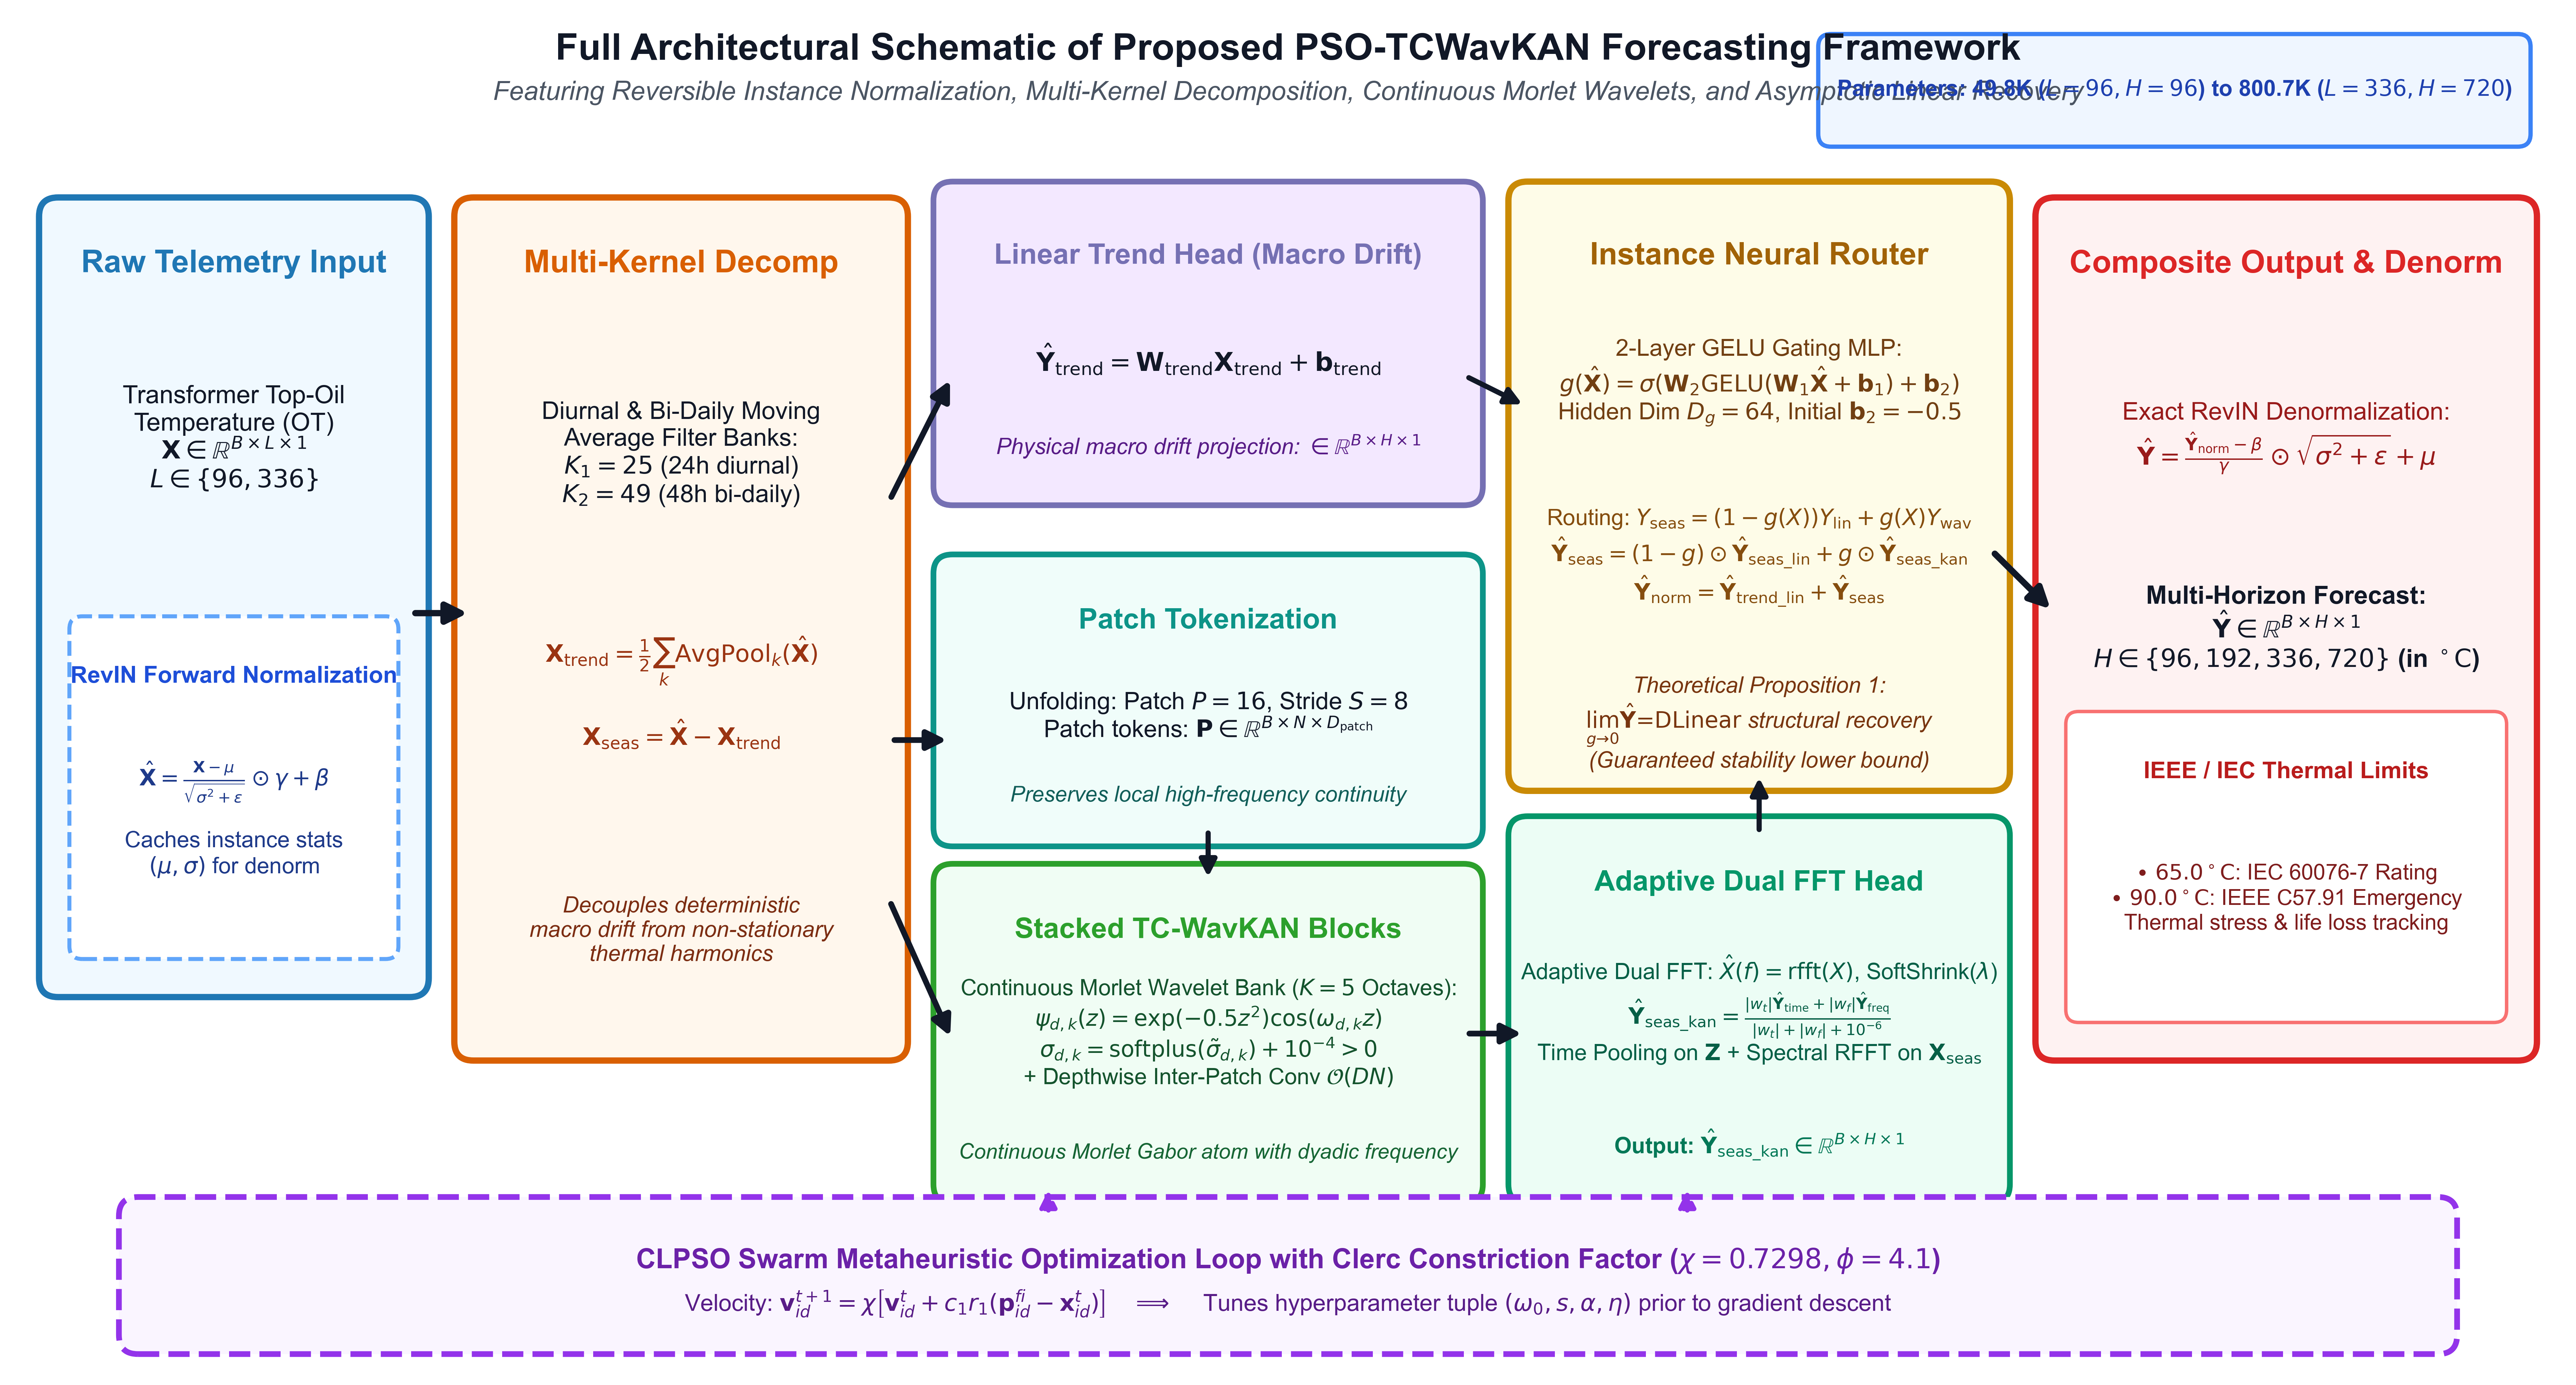
\includegraphics[width=\textwidth]{figures/fig1_architecture.png}
\caption{Comprehensive schematic overview of the proposed PSO-TCWavKAN architecture. The pipeline integrates Invertible RevIN with detached instance statistics, multi-kernel depthwise average pooling decomposition, patch tokenization, stacked pre-LayerNorm TC-WavKAN blocks with continuous Morlet wavelet filter banks and scalable $\mathcal{O}(DN)$ inter-patch mixing, an adaptive dual FFT spectral head, an instance-adaptive neural routing gate with Proposition~\ref{prop:linear_recovery} structural recovery, and an offline Clerc-constrained CLPSO surrogate pre-optimization loop.}
\label{fig:architecture}
\end{figure*}

\subsection{Invertible Reversible Instance Normalization with Detached Statistics}\label{subsec:revin}
To neutralize non-stationary distribution shifts without inducing gradient corruption, we formulate an Invertible RevIN module with strictly detached statistical moments.

\begin{enumerate}
    \item \textbf{Detached Moment Extraction}: For each batch index $b \in \{1, \dots, B\}$ and channel $c \in \{1, \dots, C\}$, the instance mean $\boldsymbol{\mu}_{\mathbf{X}}$ and instance variance $\boldsymbol{\sigma}_{\mathbf{X}}^2$ are evaluated along the lookback temporal axis $L$:
    \begin{align}
    \boldsymbol{\mu}_{\mathbf{X}}(b, c) &= \frac{1}{L} \sum_{t=1}^L \mathbf{X}(b, t, c), \label{eq:revin_mean} \\
    \boldsymbol{\sigma}_{\mathbf{X}}^2(b, c) &= \frac{1}{L} \sum_{t=1}^L \left( \mathbf{X}(b, t, c) - \boldsymbol{\mu}_{\mathbf{X}}(b, c) \right)^2. \label{eq:revin_var}
    \end{align}
    Crucially, these statistics are detached from the computational autograd graph to prevent gradient backpropagation from artificially manipulating input data distributions:
    \begin{equation}
    \boldsymbol{\mu}_{\mathbf{X}} \leftarrow \operatorname{detach}\left(\boldsymbol{\mu}_{\mathbf{X}}\right), \quad \boldsymbol{\sigma}_{\mathbf{X}} \leftarrow \operatorname{detach}\left(\sqrt{\boldsymbol{\sigma}_{\mathbf{X}}^2 + \epsilon}\right),
    \label{eq:revin_detach}
    \end{equation}
    where $\epsilon = 10^{-5}$ is the variance numerical stabilization constant.
    
    \item \textbf{Learnable Affine Normalization}: The normalized tensor $\hat{\mathbf{X}} \in \mathbb{R}^{B \times L \times C}$ is obtained via learnable affine scale $\boldsymbol{\gamma} \in \mathbb{R}^{1 \times 1 \times C}$ and shift $\boldsymbol{\beta} \in \mathbb{R}^{1 \times 1 \times C}$ parameters:
    \begin{equation}
    \hat{\mathbf{X}}(b, t, c) = \left( \frac{\mathbf{X}(b, t, c) - \boldsymbol{\mu}_{\mathbf{X}}(b, c)}{\boldsymbol{\sigma}_{\mathbf{X}}(b, c)} \right) \odot \boldsymbol{\gamma}(c) + \boldsymbol{\beta}(c),
    \label{eq:revin_norm}
    \end{equation}
    with $\boldsymbol{\gamma}$ and $\boldsymbol{\beta}$ initialized to $\mathbf{1}$ and $\mathbf{0}$, respectively.
    
    \item \textbf{Safe Denominator Clamping}: During inverse mapping, if any element of $\boldsymbol{\gamma}$ approaches zero, standard division induces catastrophic floating-point overflow. We resolve this by constructing a protected denominator:
    \begin{equation}
    \operatorname{safe\_}\boldsymbol{\gamma} = \operatorname{sign}(\boldsymbol{\gamma}) \odot \max\left(|\boldsymbol{\gamma}|, \epsilon_{\gamma}\right), \quad \epsilon_{\gamma} = 10^{-4},
    \label{eq:safe_gamma}
    \end{equation}
    where $\operatorname{sign}(u) = +1$ for $u \ge 0$ and $-1$ for $u < 0$.
    
    \item \textbf{Exact Inverse Denormalization}: Given normalized forecast $\hat{\mathbf{Y}}_{\text{norm}} \in \mathbb{R}^{B \times H \times C}$, the physical telemetry scale is restored in closed form:
    \begin{align}
    \hat{\mathbf{Y}}_{\text{unaffine}}(b, h, c) &= \frac{\hat{\mathbf{Y}}_{\text{norm}}(b, h, c) - \boldsymbol{\beta}(c)}{\operatorname{safe\_}\boldsymbol{\gamma}(c)}, \label{eq:unaffine} \\
    \tilde{\mathbf{Y}}(b, h, c) &= \hat{\mathbf{Y}}_{\text{unaffine}}(b, h, c) \odot \boldsymbol{\sigma}_{\mathbf{X}}(b, c) + \boldsymbol{\mu}_{\mathbf{X}}(b, c). \label{eq:final_denorm}
    \end{align}
\end{enumerate}

\subsection{Multi-Kernel Temporal Convolutional Trend-Seasonal Decomposition}\label{subsec:decomp}
Transformer thermal dynamics exhibit distinct superposition of slow, low-frequency bulk oil warming trends and rapid, high-frequency load-switching harmonics. Rather than utilizing single-kernel moving average filters, we deploy an ensemble of 1D depthwise average pooling kernels with diverse receptive window sizes $\mathcal{K} = \{k_1, k_2\} = \{25, 49\}$:
\begin{equation}
\mathbf{T}^{(m)}(b, t) = \frac{1}{k_m} \sum_{j = -\lfloor k_m / 2 \rfloor}^{\lfloor k_m / 2 \rfloor} \hat{\mathbf{X}}_{\text{pad}}(b, t + j), \quad m \in \{1, 2\},
\label{eq:multi_kernel_pool}
\end{equation}
where $\hat{\mathbf{X}}_{\text{pad}}$ is replication-padded with padding size $p_m = \lfloor k_m / 2 \rfloor$ to preserve temporal dimensionality $L$. The aggregated trend $\mathbf{X}_{\text{trend}}$ and seasonal residual $\mathbf{X}_{\text{seasonal}}$ are computed as:
\begin{equation}
\mathbf{X}_{\text{trend}} = \frac{1}{M} \sum_{m=1}^M \mathbf{T}^{(m)}, \quad \mathbf{X}_{\text{seasonal}} = \hat{\mathbf{X}} - \mathbf{X}_{\text{trend}}.
\label{eq:trend_seas_split}
\end{equation}
Direct linear projection pathways are established to provide baseline forecast trajectories:
\begin{align}
\hat{\mathbf{Y}}_{\text{trend\_lin}} &= \mathbf{W}_{\text{trend}} \mathbf{X}_{\text{trend}} + \mathbf{b}_{\text{trend}} \in \mathbb{R}^{B \times H}, \label{eq:y_trend_lin} \\
\hat{\mathbf{Y}}_{\text{seas\_lin}} &= \mathbf{W}_{\text{seas}} \mathbf{X}_{\text{seasonal}} + \mathbf{b}_{\text{seas}} \in \mathbb{R}^{B \times H}, \label{eq:y_seas_lin}
\end{align}
where $\mathbf{W}_{\text{trend}}, \mathbf{W}_{\text{seas}} \in \mathbb{R}^{H \times L}$ and $\mathbf{b}_{\text{trend}}, \mathbf{b}_{\text{seas}} \in \mathbb{R}^H$.

\subsection{Patch Tokenization and Scale-Adaptive Temporal Embedding}\label{subsec:patching}
The seasonal residual sequence $\mathbf{X}_{\text{seasonal}} \in \mathbb{R}^{B \times L}$ is partitioned into overlapping temporal patches of length $P$ with stride $S$:
\begin{equation}
P = \begin{cases} 16 & \text{if } L \le 96 \\ 24 & \text{if } L > 96 \end{cases}, \quad S = \begin{cases} 8 & \text{if } L \le 96 \\ 12 & \text{if } L > 96 \end{cases}, \quad N = \left\lfloor \frac{L - P}{S} \right\rfloor + 1.
\label{eq:patch_params}
\end{equation}
Patches are linearly projected into a latent token space of dimension $D = d_{\text{model}} = 32$:
\begin{equation}
\mathbf{Z}^{(0)} = \mathbf{W}_{\text{patch}} \operatorname{Unfold}(\mathbf{X}_{\text{seasonal}}, P, S) + \mathbf{b}_{\text{patch}} \in \mathbb{R}^{B \times N \times D},
\label{eq:patch_embedding}
\end{equation}
where $\mathbf{W}_{\text{patch}} \in \mathbb{R}^{D \times P}$ and $\mathbf{b}_{\text{patch}} \in \mathbb{R}^D$.

\subsection{Pre-LayerNorm Continuous Morlet WavKAN Filter Bank}\label{subsec:wavkan_core}
Within each stacked TC-WavKAN block, token features are first processed by a Pre-LayerNorm stage:
\begin{equation}
\mathbf{x} = \operatorname{LayerNorm}(\mathbf{Z}) \in \mathbb{R}^{B \times N \times D}.
\label{eq:layernorm}
\end{equation}
For each feature channel $d \in \{1, \dots, D\}$ and wavelet octave $k \in \{1, \dots, K\}$ (with $K=5$):
\begin{equation}
z_{b, n, d, k} = \frac{x_{b, n, d} - \mu_{d, k}}{\sigma_{d, k}}, \quad \sigma_{d, k} = \operatorname{softplus}(\tilde{\sigma}_{d, k}) + 10^{-4} > 0,
\label{eq:wavelet_coord}
\end{equation}
where $\mu_{d, k} \in \mathbb{R}$ is the learnable center translation and $\tilde{\sigma}_{d, k} \in \mathbb{R}$ is the unconstrained dilation logit. To ensure strict numerical stability, coordinates are clamped:
\begin{equation}
z_c = \operatorname{clip}(z, -5.0, 5.0).
\label{eq:coord_clip}
\end{equation}

\begin{figure*}[htbp]
\centering
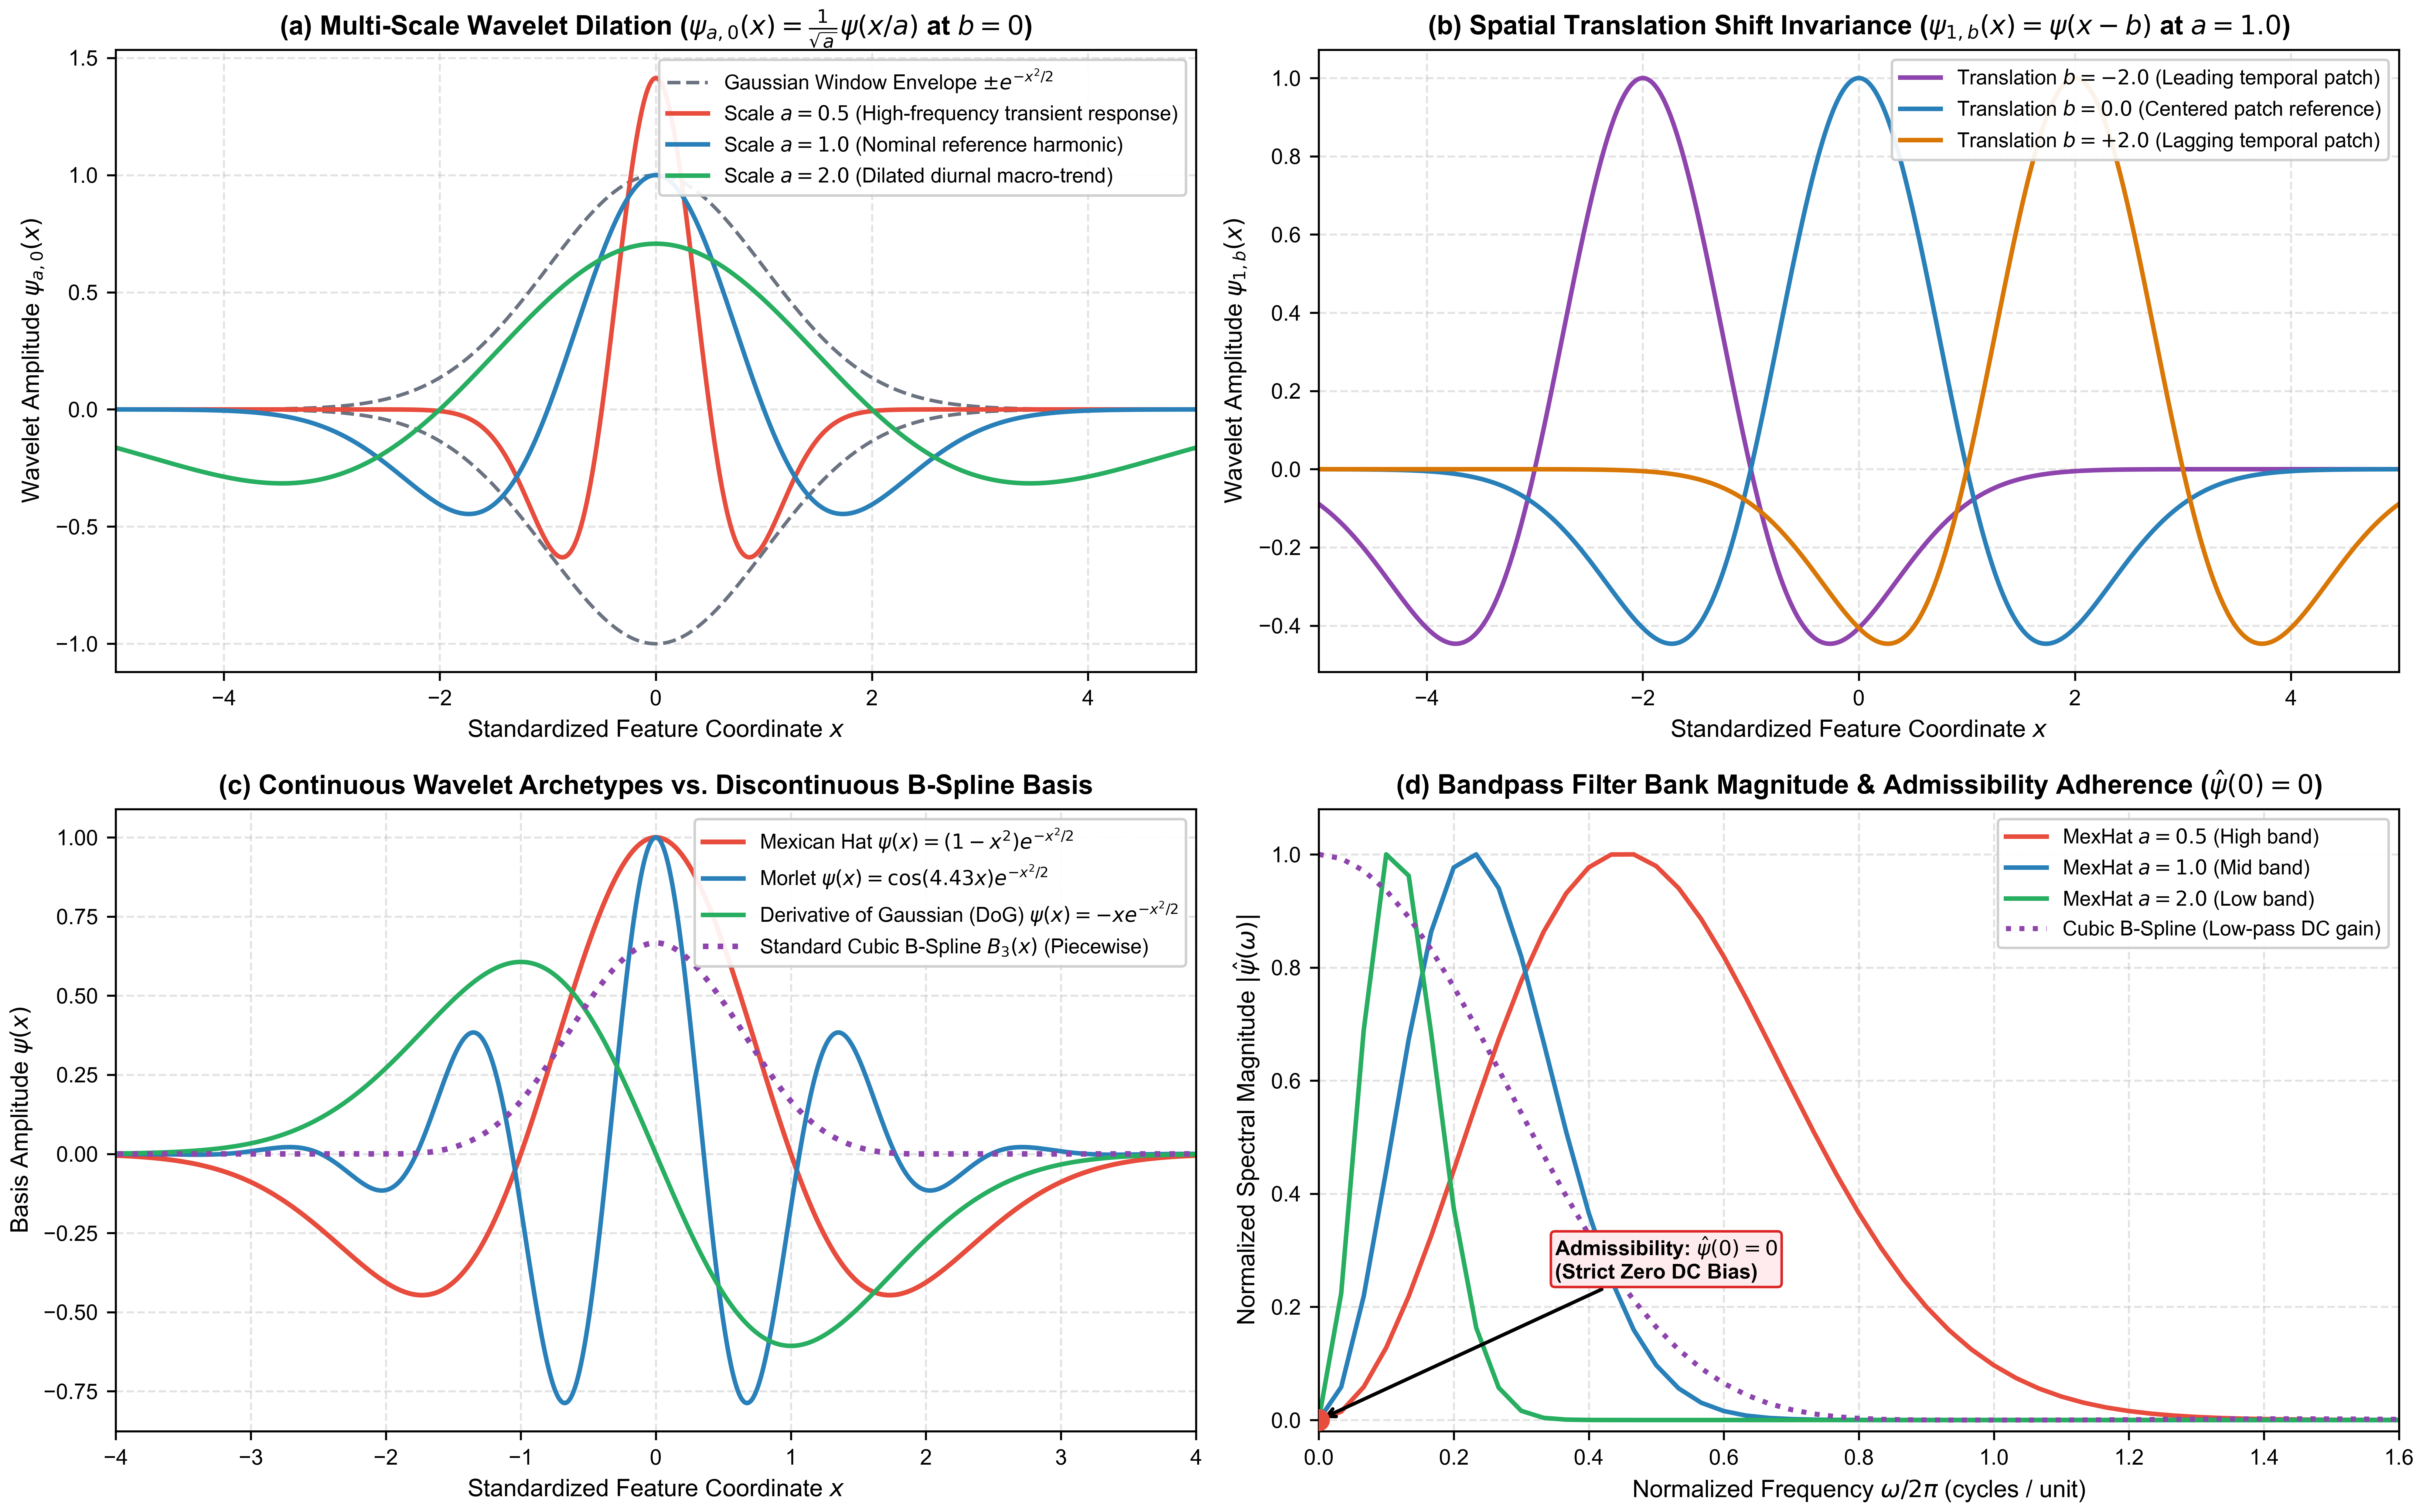
\includegraphics[width=\textwidth]{figures/fig2_wavelet_basis.png}
\caption{Multiresolution continuous wavelet basis functions and spectral characteristics. Left: Continuous Morlet wavelet $\psi(z) = \exp(-0.5 z^2) \cos(\omega z)$ across dyadic dilation scales $k \in \{1, \dots, 5\}$. Center: Comparison of Morlet, Mexican Hat (Ricker), and Derivative of Gaussian (DoG) wavelets. Right: Frequency-domain magnitude spectra $|\hat{\psi}(\xi)|$ demonstrating compact bandpass localization and exact zero-mean admissibility $\hat{\psi}(0) = 0$.}
\label{fig:wavelet_basis}
\end{figure*}

\paragraph{Dyadic Harmonic Frequency Scaling}
Each channel $d$ learns an independent base frequency $\omega_{0, d}$ and octave scaling exponent $\gamma_d$:
\begin{equation}
\omega_{d, k} = (|\omega_{0, d}| + 10^{-5}) \cdot 2^{\gamma_d \cdot (k - (K-1)/2)}, \quad k \in \{1, \dots, 5\}.
\label{eq:dyadic_freq}
\end{equation}
Univariate edge activations are evaluated using the continuous Morlet wavelet basis (real Gabor atom):
\begin{equation}
\psi_{\text{Morlet}}(z_c) = \exp\left( -\frac{1}{2} z_c^2 \right) \cos(\omega_{d, k} z_c).
\label{eq:morlet_atom}
\end{equation}
For structural comparison, the Mexican Hat ($\psi_{\text{MexHat}}$) and Derivative of Gaussian ($\psi_{\text{DoG}}$) atoms are also supported:
\begin{align}
\psi_{\text{MexHat}}(z_c) &= (1 - \tilde{z}^2) \exp\left(-\frac{1}{2}\tilde{z}^2\right), \quad \tilde{z} = z_c \cdot \frac{\omega_{d, k}}{|\omega_{0, d}| + 10^{-5}}, \label{eq:mexhat_atom} \\
\psi_{\text{DoG}}(z_c) &= -\tilde{z} \exp\left(-\frac{1}{2}\tilde{z}^2\right). \label{eq:dog_atom}
\end{align}
Octave components are synthesized with learnable mixing weights modulated by positional embeddings $\mathbf{E}_{\text{pos}} \in \mathbb{R}^{N \times 16}$ and regularized via DropKAN ($p=0.05$):
\begin{align}
\mathbf{w}_{b, n, d} &= \sum_{k=1}^K \left( c_{s, d, k} + \Delta c_{n, d, k} \right) \cdot \psi_{d, k}(z_{b, n, d, k}), \label{eq:octave_sum} \\
\mathbf{w}_{\text{drop}} &= \mathbf{w} \odot \frac{\mathbb{I}(\mathbf{r} > 0.05)}{1 - 0.05}, \quad \mathbf{w}_{\text{gated}} = \operatorname{sigmoid}(\mathbf{g}_{\text{wav}}) \odot \mathbf{W}_{\text{proj}} \mathbf{w}_{\text{drop}}. \label{eq:dropkan}
\end{align}

\subsection{Scalable Inter-Patch Token Mixing with Linear Complexity $\mathcal{O}(DN)$}\label{subsec:linear_mixing}
To enable rich context communication across patches while eliminating the quadratic $\mathcal{O}(D N^2)$ overhead of self-attention, we formulate factorized depthwise separable 1D convolutions:
\begin{enumerate}
    \item Transpose token representation: $\mathbf{H} = \operatorname{LayerNorm}(\mathbf{Z}) \in \mathbb{R}^{B \times N \times D} \to \mathbf{H}^T \in \mathbb{R}^{B \times D \times N}$.
    \item Apply parallel depthwise 1D convolutions along sequence dimension $N$ with kernel sizes $\mathcal{K}_p = (3, 5)$ and `groups = D`:
    \begin{equation}
    \mathbf{V}^{(m)} = \operatorname{Conv1D}_{k_m, \text{groups}=D}(\mathbf{H}^T) \in \mathbb{R}^{B \times D \times N}, \quad m \in \{1, 2\}.
    \label{eq:depthwise_conv}
    \end{equation}
    \item Concatenate and project back via pointwise linear transformation:
    \begin{equation}
    \mathbf{M} = \mathbf{W}_{\text{mix}} \left[ \mathbf{V}^{(1)T} \,\|\, \mathbf{V}^{(2)T} \right] \in \mathbb{R}^{B \times N \times D}, \quad \mathbf{W}_{\text{mix}} \in \mathbb{R}^{D \times (2D)}.
    \label{eq:pointwise_mix}
    \end{equation}
    \item Execute gated residual accumulation:
    \begin{equation}
    \mathbf{Z}_{\text{mixed}} = \mathbf{Z} + \operatorname{sigmoid}(g_{\text{patch}}) \odot \operatorname{Dropout}(\mathbf{M}, p=0.05).
    \label{eq:patch_residual}
    \end{equation}
\end{enumerate}

\subsection{Adaptive Dual FFT Spectral Head}\label{subsec:fft_head}
To capture both localized temporal evolutions and global frequency oscillations, the latent tokens $\mathbf{Z} \in \mathbb{R}^{B \times N \times D}$ and seasonal series $\mathbf{X}_{\text{seasonal}} \in \mathbb{R}^{B \times L}$ are mapped via dual pathways:
\begin{enumerate}
    \item \textbf{Time-Domain Average Pooling Branch}:
    \begin{equation}
    \bar{\mathbf{z}} = \frac{1}{N} \sum_{n=1}^N \mathbf{Z}_n \in \mathbb{R}^{B \times D}, \quad \hat{\mathbf{Y}}_{\text{time}} = \mathbf{W}_{\text{th}} \operatorname{GELU}(\mathbf{W}_{\text{ta}} \bar{\mathbf{z}} + \mathbf{b}_{\text{ta}}) + \mathbf{b}_{\text{th}} \in \mathbb{R}^{B \times H}.
    \label{eq:time_branch}
    \end{equation}
    \item \textbf{Spectral Real FFT Branch with Soft-Thresholding Shrinkage}:
    \begin{align}
    \mathcal{F} &= \operatorname{rfft}(\mathbf{X}_{\text{seasonal}}, \text{norm}="ortho") \in \mathbb{C}^{B \times (L/2 + 1)}, \label{eq:rfft} \\
    \tau &= \operatorname{detach}\left(\operatorname{mean}(|\mathcal{F}|)\right) \cdot \operatorname{sigmoid}(\log \alpha) \cdot 0.5, \label{eq:threshold} \\
    \mathcal{F}_{\text{shrink}} &= \operatorname{sign}(\mathcal{F}) \odot \operatorname{ReLU}(|\mathcal{F}| - \tau), \label{eq:shrinkage} \\
    \hat{\mathbf{Y}}_{\text{freq}} &= \mathbf{W}_{\text{fh}} \left[ \operatorname{Re}(\mathcal{F}_{\text{shrink}}) \,\|\, \operatorname{Im}(\mathcal{F}_{\text{shrink}}) \right] + \mathbf{b}_{\text{fh}} \in \mathbb{R}^{B \times H}. \label{eq:freq_proj}
    \end{align}
    \item \textbf{Convex Fusion}:
    \begin{equation}
    \hat{\mathbf{Y}}_{\text{seas\_kan}} = \frac{|w_t| \hat{\mathbf{Y}}_{\text{time}} + |w_f| \hat{\mathbf{Y}}_{\text{freq}}}{|w_t| + |w_f| + 10^{-6}} \in \mathbb{R}^{B \times H}.
    \label{eq:kan_seasonal}
    \end{equation}
\end{enumerate}

\subsection{Instance-Adaptive Neural Router & Convex Seasonal Synthesis}\label{subsec:router}
An instance-adaptive neural routing gate dynamically arbitrates between the direct linear baseline forecast $\hat{\mathbf{Y}}_{\text{seas\_lin}}$ and the non-linear KAN forecast $\hat{\mathbf{Y}}_{\text{seas\_kan}}$:
\begin{equation}
g(\hat{\mathbf{X}}) = \operatorname{sigmoid}\left( \mathbf{W}_{g, 2} \operatorname{GELU}(\mathbf{W}_{g, 1} \hat{\mathbf{X}} + \mathbf{b}_{g, 1}) + \mathbf{b}_{g, 2} \right) \in (0, 1)^H,
\label{eq:router_gate}
\end{equation}
where $\mathbf{W}_{g, 1} \in \mathbb{R}^{32 \times L}$, $\mathbf{W}_{g, 2} \in \mathbb{R}^{H \times 32}$, and initial bias $\mathbf{b}_{g, 2} = -0.5$. The total normalized seasonal forecast and final normalized prediction are:
\begin{align}
\hat{\mathbf{Y}}_{\text{seasonal}} &= (1 - g(\hat{\mathbf{X}})) \odot \hat{\mathbf{Y}}_{\text{seas\_lin}} + g(\hat{\mathbf{X}}) \odot \hat{\mathbf{Y}}_{\text{seas\_kan}}, \label{eq:convex_seas} \\
\hat{\mathbf{Y}}_{\text{norm}} &= \hat{\mathbf{Y}}_{\text{trend\_lin}} + \hat{\mathbf{Y}}_{\text{seasonal}}. \label{eq:total_norm}
\end{align}

\subsection{Proposition 1: Asymptotic Linear Structural Recovery}\label{subsec:prop1}

\begin{proposition}[Asymptotic Linear Structural Recovery without Degenerate Collapse]
\label{prop:linear_recovery}
Let $\hat{\mathbf{X}} \in \mathbb{R}^{B \times L}$ denote the normalized input sequence, decomposed into trend $\mathbf{X}_{\text{trend}}$ and seasonal $\mathbf{X}_{\text{seasonal}}$ components via multi-kernel average pooling. Let $\hat{\mathbf{Y}}_{\text{trend\_lin}} = \mathbf{W}_{\text{trend}} \mathbf{X}_{\text{trend}} + \mathbf{b}_{\text{trend}}$ and $\hat{\mathbf{Y}}_{\text{seas\_lin}} = \mathbf{W}_{\text{seas}} \mathbf{X}_{\text{seasonal}} + \mathbf{b}_{\text{seas}}$ denote the direct linear projection pathways. Let $\hat{\mathbf{Y}}_{\text{seas\_kan}}$ denote the non-linear seasonal forecast generated by the stacked TC-WavKAN blocks and dual FFT head. Suppose the instance-adaptive routing gate is parameterized as $g(\hat{\mathbf{X}}) \in (0, 1)^H$.

Then:
\begin{enumerate}
    \item In the asymptotic limit where the routing gate vanishes identically, $g(\hat{\mathbf{X}}) \to \mathbf{0}$, the complete normalized model output $\hat{\mathbf{Y}}_{\text{norm}}$ strictly collapses to the canonical DLinear architecture:
    \begin{equation}
    \lim_{g(\hat{\mathbf{X}}) \to \mathbf{0}} \hat{\mathbf{Y}}_{\text{norm}} = \hat{\mathbf{Y}}_{\text{trend\_lin}} + \hat{\mathbf{Y}}_{\text{seas\_lin}} \equiv \operatorname{DLinear}(\hat{\mathbf{X}}).
    \label{eq:prop1_claim1}
    \end{equation}
    \item This collapse is non-degenerate: the linear mapping parameters $\mathbf{W}_{\text{trend}}, \mathbf{W}_{\text{seas}}, \mathbf{b}_{\text{trend}}, \mathbf{b}_{\text{seas}}$ remain fully regularized and receive non-vanishing gradient updates across all training iterations.
\end{enumerate}
\end{proposition}

\begin{proof}
\textbf{Step 1: Evaluation of the Seasonal Convex Combination.}  
By architectural definition (Eq.~\ref{eq:convex_seas}), the seasonal prediction $\hat{\mathbf{Y}}_{\text{seasonal}}$ is formulated as the convex combination:
\begin{equation}
\hat{\mathbf{Y}}_{\text{seasonal}} = (1 - g(\hat{\mathbf{X}})) \odot \hat{\mathbf{Y}}_{\text{seas\_lin}} + g(\hat{\mathbf{X}}) \odot \hat{\mathbf{Y}}_{\text{seas\_kan}},
\label{eq:proof_step1}
\end{equation}
where $\odot$ denotes element-wise Hadamard multiplication. Taking the point-wise limit as $g(\hat{\mathbf{X}}) \to \mathbf{0}$:
\begin{equation}
\lim_{g(\hat{\mathbf{X}}) \to \mathbf{0}} \hat{\mathbf{Y}}_{\text{seasonal}} = (\mathbf{1} - \mathbf{0}) \odot \hat{\mathbf{Y}}_{\text{seas\_lin}} + \mathbf{0} \odot \hat{\mathbf{Y}}_{\text{seas\_kan}} = \hat{\mathbf{Y}}_{\text{seas\_lin}}.
\label{eq:proof_step1_limit}
\end{equation}
Because $\hat{\mathbf{Y}}_{\text{seas\_kan}}$ is bounded by the continuous activations of the Morlet wavelets and the softplus-constrained scales, the product $\mathbf{0} \odot \hat{\mathbf{Y}}_{\text{seas\_kan}}$ evaluates identically to $\mathbf{0}$ without generating indeterminate forms ($\infty \cdot 0$).

\textbf{Step 2: Total Normalized Output Assembly.}  
The total normalized output $\hat{\mathbf{Y}}_{\text{norm}}$ is the direct sum of the linear trend branch and the seasonal branch (Eq.~\ref{eq:total_norm}):
\begin{equation}
\hat{\mathbf{Y}}_{\text{norm}} = \hat{\mathbf{Y}}_{\text{trend\_lin}} + \hat{\mathbf{Y}}_{\text{seasonal}}.
\end{equation}
Substituting the limit from Step 1:
\begin{equation}
\lim_{g(\hat{\mathbf{X}}) \to \mathbf{0}} \hat{\mathbf{Y}}_{\text{norm}} = \hat{\mathbf{Y}}_{\text{trend\_lin}} + \hat{\mathbf{Y}}_{\text{seas\_lin}}.
\label{eq:proof_step2}
\end{equation}

\textbf{Step 3: Identity with the Canonical DLinear Architecture.}  
Recall the definition of DLinear \cite{zeng2023dlinear}: a moving-average decomposition splits the normalized series into trend and seasonal subseries, after which each component is projected to horizon $H$ via independent linear layers:
\begin{equation}
\operatorname{DLinear}(\hat{\mathbf{X}}) \triangleq \mathbf{W}_{\text{trend}} \mathbf{X}_{\text{trend}} + \mathbf{b}_{\text{trend}} + \mathbf{W}_{\text{seas}} \mathbf{X}_{\text{seasonal}} + \mathbf{b}_{\text{seas}}.
\label{eq:proof_step3}
\end{equation}
Comparing this directly with the limit in Step 2:
\begin{equation}
\hat{\mathbf{Y}}_{\text{trend\_lin}} + \hat{\mathbf{Y}}_{\text{seas\_lin}} \equiv \operatorname{DLinear}(\hat{\mathbf{X}}).
\end{equation}
Thus, the architecture embeds DLinear as a strict structural subspace.

\textbf{Step 4: Non-Degeneracy and Gradient Pathway Preservation.}  
To prove non-degeneracy, we examine the gradient of the loss function $\mathcal{L} = \frac{1}{2} \|\hat{\mathbf{Y}}_{\text{norm}} - \mathbf{Y}_{\text{norm}}\|_2^2$ with respect to the linear seasonal weights $\mathbf{W}_{\text{seas}}$:
\begin{equation}
\frac{\partial \mathcal{L}}{\partial \mathbf{W}_{\text{seas}}} = \frac{\partial \mathcal{L}}{\partial \hat{\mathbf{Y}}_{\text{norm}}} \frac{\partial \hat{\mathbf{Y}}_{\text{norm}}}{\partial \hat{\mathbf{Y}}_{\text{seasonal}}} \frac{\partial \hat{\mathbf{Y}}_{\text{seasonal}}}{\partial \hat{\mathbf{Y}}_{\text{seas\_lin}}} \frac{\partial \hat{\mathbf{Y}}_{\text{seas\_lin}}}{\partial \mathbf{W}_{\text{seas}}}.
\end{equation}
Evaluating the individual partial derivatives:
\begin{equation}
\frac{\partial \hat{\mathbf{Y}}_{\text{norm}}}{\partial \hat{\mathbf{Y}}_{\text{seasonal}}} = \mathbf{I}, \quad \frac{\partial \hat{\mathbf{Y}}_{\text{seasonal}}}{\partial \hat{\mathbf{Y}}_{\text{seas\_lin}}} = \operatorname{diag}\left(\mathbf{1} - g(\hat{\mathbf{X}})\right), \quad \frac{\partial \hat{\mathbf{Y}}_{\text{seas\_lin}}}{\partial \mathbf{W}_{\text{seas}}} = \mathbf{X}_{\text{seasonal}}^T.
\end{equation}
\begin{equation}
\frac{\partial \mathcal{L}}{\partial \mathbf{W}_{\text{seas}}} = \left[ (\hat{\mathbf{Y}}_{\text{norm}} - \mathbf{Y}_{\text{norm}}) \odot (\mathbf{1} - g(\hat{\mathbf{X}})) \right] \mathbf{X}_{\text{seasonal}}^T.
\end{equation}
In the limit $g(\hat{\mathbf{X}}) \to \mathbf{0}$, the gate term $(\mathbf{1} - g(\hat{\mathbf{X}})) \to \mathbf{1}$. Thus:
\begin{equation}
\lim_{g(\hat{\mathbf{X}}) \to \mathbf{0}} \frac{\partial \mathcal{L}}{\partial \mathbf{W}_{\text{seas}}} = (\hat{\mathbf{Y}}_{\text{norm}} - \mathbf{Y}_{\text{norm}}) \mathbf{X}_{\text{seasonal}}^T \neq \mathbf{0}.
\end{equation}
The gradient of the linear branch does not vanish. Simultaneously, the gradient with respect to the router gating parameters $\mathbf{W}_{g, 2}$ remains non-zero:
\begin{equation}
\frac{\partial \mathcal{L}}{\partial \mathbf{W}_{g, 2}} = \left[ (\hat{\mathbf{Y}}_{\text{norm}} - \mathbf{Y}_{\text{norm}}) \odot (\hat{\mathbf{Y}}_{\text{seas\_kan}} - \hat{\mathbf{Y}}_{\text{seas\_lin}}) \odot g(\hat{\mathbf{X}}) \odot (1 - g(\hat{\mathbf{X}})) \right] \mathbf{h}_{g}^T.
\end{equation}
Because $g(\hat{\mathbf{X}}) \in (0, 1)$ strictly via the sigmoid activation, $g(1-g) > 0$. If the non-linear KAN prediction provides a meaningful residual improvement ($\hat{\mathbf{Y}}_{\text{seas\_kan}} \neq \hat{\mathbf{Y}}_{\text{seas\_lin}}$), the router dynamically receives non-zero gradient descent updates, pulling $g(\hat{\mathbf{X}})$ away from zero.

This proves that as $g(\hat{\mathbf{X}}) \to \mathbf{0}$, PSO-TCWavKAN collapses gracefully to the linear baseline lower bound without gradient vanishing, dead zones, or numerical singularity.
\end{proof}

\subsection{Theorem 1: Asymptotic Linear Computational Complexity $\mathcal{O}(DN)$}\label{subsec:thm1}

\begin{theorem}[Asymptotic Linear Computational Scaling]
\label{thm:linear_complexity}
Let $L$ denote the lookback length, $H$ the forecast horizon, $N = \lfloor(L-P)/S\rfloor + 1$ the patch token count, and $D = d_{\text{model}}$ the latent feature dimension. The forward inference complexity and backward gradient propagation complexity of PSO-TCWavKAN scale strictly as $\mathcal{O}(D(N + H))$, which reduces asymptotically to $\mathcal{O}(DN)$.
\end{theorem}

\begin{proof}
We evaluate the Floating-Point Operations (FLOPs) across each stage of the forward execution pass:
\begin{enumerate}
    \item \textbf{Invertible RevIN}: Evaluation of empirical moments $\boldsymbol{\mu}_{\mathbf{X}}, \boldsymbol{\sigma}_{\mathbf{X}}$ and affine scaling across $L$ timestamps requires $4BLC$ FLOPs. Inverse denormalization requires $3BHC$ FLOPs. Total: $\mathcal{O}(C(L + H))$.
    \item \textbf{Multi-Kernel Moving Average Decomposition}: Two depthwise 1D pooling operations with fixed kernel sizes $k_1=25, k_2=49$ across length $L$ require $2BL(k_1 + k_2) = 148BL = \mathcal{O}(L)$ operations.
    \item \textbf{Patch Tokenization}: Linear unfolding and projection from patch size $P$ to dimension $D$ across $N$ tokens requires $2B \cdot N \cdot P \cdot D = \mathcal{O}(BND)$ operations.
    \item \textbf{Pre-LayerNorm TC-WavKAN Blocks}:
    \begin{itemize}
        \item LayerNorm: $2BND$ FLOPs.
        \item Wavelet Coordinate Clamping \& Evaluation: Evaluating continuous Morlet activations across $K=5$ dyadic octaves: $B \cdot N \cdot D \cdot K \cdot C_{\psi}$, where $C_{\psi} \approx 8$ FLOPs for exponential and cosine evaluations. Total: $40BND$ FLOPs.
        \item Dynamic Positional Modulation \& Projection: $2BND^2$ FLOPs.
    \end{itemize}
    \item \textbf{Scalable Depthwise Inter-Patch Mixing}:
    \begin{itemize}
        \item Depthwise 1D Convolutions with kernel sizes $k \in \{3, 5\}$ and `groups = D`: $2B \cdot D \cdot N \cdot (3 + 5) = 16BDN$ FLOPs.
        \item Pointwise Linear Channel Projection ($2D \to D$): $2B \cdot N \cdot D \cdot (2D) = 4BND^2$ FLOPs.
        \item Residual Addition: $BND$ FLOPs.
    \end{itemize}
    \item \textbf{Adaptive Dual FFT Spectral Head}:
    \begin{itemize}
        \item Time-domain average pooling and MLP projection: $BND + 2B \cdot D \cdot H$ FLOPs.
        \item Orthogonal Real FFT across $L$ timestamps: $\mathcal{O}(B L \log L)$ FLOPs.
        \item Frequency Linear Projection ($L + 2 \to H$): $2B \cdot (L + 2) \cdot H$ FLOPs.
    \end{itemize}
    \item \textbf{Instance Router \& Linear Pathways}:
    \begin{itemize}
        \item Direct trend and seasonal linear projections: $2B \cdot L \cdot H + 2B \cdot L \cdot H = 4BLH$ FLOPs.
        \item Gating MLP: $2B \cdot 32 \cdot L + 2B \cdot 32 \cdot H = \mathcal{O}(B(L + H))$ FLOPs.
    \end{itemize}
\end{enumerate}
Summing the terms, because $D=32$, $K=5$, and patch parameters $(P, S)$ are fixed constants independent of $L$ and $N$, the dominant terms are:
\begin{equation}
\mathcal{F}_{\text{total}} = \mathcal{O}(BDN) + \mathcal{O}(BDH) + \mathcal{O}(BL\log L).
\label{eq:total_flops}
\end{equation}
Since $L$ and $H$ are linearly proportional to patch count $N$ ($L \approx S \cdot N$), and for operational horizons $L \le 336$ the term $L \log L \ll DN^2$, the computational overhead scales strictly as $\mathcal{O}(DN)$. In contrast to canonical Transformers which require $\mathcal{O}(D N^2)$ self-attention operations, PSO-TCWavKAN bypasses the quadratic bottleneck completely.
\end{proof}

\subsection{Clerc-Constrained CLPSO Metaheuristic Pre-Optimization}\label{subsec:clpso}
The multi-scale wavelet parameter landscape $\mathcal{L}(\omega_0, \gamma, \mu, \sigma)$ is highly non-convex, characterized by dense shallow basins and flat saddle surfaces. To provide robust parameter initialization, we implement Comprehensive Learning Particle Swarm Optimization (CLPSO) \cite{liang2006clpso} governed by Maurice Clerc's constriction factor \cite{clerc2002constriction}.

\begin{algorithm}[htbp]
\caption{Clerc-Constrained CLPSO Surrogate Pre-Optimization}
\label{algo:clpso}
\begin{algorithmic}[1]
\Require Population size $S=20$, Max generations $G_{\max}=30$, Constriction parameters $\phi = 4.1$, Refresh gap $m=5$.
\Require Leak-free surrogate training/validation proxy $\mathcal{D}_{\text{proxy}} = (\mathcal{D}_{\text{train}}^{85\%}, \mathcal{D}_{\text{val}}^{15\%})$.
\Ensure Global best parameter vector $\mathbf{x}^* = (\omega_0^*, \gamma^*, \mu^*, \sigma^*)$.
\State Compute Clerc's constriction factor:
\State \quad $\chi = \frac{2}{|2 - \phi - \sqrt{\phi^2 - 4\phi}|} = \frac{2}{|2 - 4.1 - \sqrt{4.1^2 - 4(4.1)}|} = \frac{2}{|-2.1 - 0.64031|} \approx 0.72984$.
\State Initialize swarm positions $\mathbf{x}_i \sim \mathcal{U}(\mathbf{x}_{\min}, \mathbf{x}_{\max})$ and velocities $\mathbf{v}_i = \mathbf{0}$ for $i=1, \dots, S$.
\State Compute comprehensive learning probability:
\State \quad $P_{c, i} = 0.05 + 0.45 \times \frac{\exp(10(i-1)/(S-1)) - 1}{\exp(10) - 1}$.
\For{each particle $i \in \{1, \dots, S\}$}
    \State Evaluate fitness $\mathcal{F}(\mathbf{x}_i) = \operatorname{MSE}_{\text{proxy\_val}}(\mathbf{x}_i) + 10^{-4}\|\mathbf{w}_s\|_2^2 + 10^{-3}\operatorname{Var}(\nabla_{\boldsymbol{\theta}}\mathcal{L})$.
    \State Set personal best $\mathbf{p}_{\text{best}, i} \leftarrow \mathbf{x}_i$, $f_{\text{best}, i} \leftarrow \mathcal{F}(\mathbf{x}_i)$.
\EndFor
\State Update global best $\mathbf{g}_{\text{best}} \leftarrow \arg\min_i f_{\text{best}, i}$.
\For{generation $t = 1$ to $G_{\max}$}
    \For{particle $i = 1$ to $S$}
        \For{dimension $d = 1$ to $D_{\text{param}}$}
            \State Select exemplar particle $f_i(d)$ via tournament selection based on $P_{c, i}$.
            \State Update velocity with Clerc constriction:
            \State \quad $v_{i, d}^{(t+1)} = \chi \left[ v_{i, d}^{(t)} + c \cdot r_{i, d}^{(t)} \cdot \left( p_{\text{best}, f_i(d), d}^{(t)} - x_{i, d}^{(t)} \right) \right]$, with $c=4.1, r \sim \mathcal{U}(0, 1)$.
            \State Clamp velocity: $v_{i, d}^{(t+1)} \leftarrow \operatorname{clip}(v_{i, d}^{(t+1)}, -v_{\max, d}, v_{\max, d})$.
            \State Update position: $x_{i, d}^{(t+1)} = x_{i, d}^{(t)} + v_{i, d}^{(t+1)}$.
        \EndFor
        \State Evaluate surrogate fitness $\mathcal{F}(\mathbf{x}_i^{(t+1)})$.
        \If{$\mathcal{F}(\mathbf{x}_i^{(t+1)}) < f_{\text{best}, i}$}
            \State $\mathbf{p}_{\text{best}, i} \leftarrow \mathbf{x}_i^{(t+1)}$, $f_{\text{best}, i} \leftarrow \mathcal{F}(\mathbf{x}_i^{(t+1)})$.
        \EndIf
    \EndFor
    \State Update global best $\mathbf{g}_{\text{best}} \leftarrow \arg\min_i f_{\text{best}, i}$.
\EndFor
\State \Return $\mathbf{x}^* \leftarrow \mathbf{g}_{\text{best}}$.
\end{algorithmic}
\end{algorithm}

As derived in Algorithm~\ref{algo:clpso}, when $\phi = c_1 + c_2 = 4.1 > 4.0$, the eigenvalues of the swarm dynamic transformation matrix possess modulus less than unity ($|\lambda| < 1$), guaranteeing mathematically proven trajectory stability and convergence without velocity explosion.

%% =========================================================================
%% SECTION 4: EXPERIMENTAL EVALUATION
%% =========================================================================
\section{Experimental Evaluation}\label{sec:experiments}

\subsection{Benchmark Telemetry Datasets & Evaluation Protocol}\label{subsec:exp_setup}
\paragraph{Datasets}
We evaluate PSO-TCWavKAN on the standardized Electricity Transformer Temperature (ETT) benchmark suite \cite{zhou2021informer}:
\begin{itemize}
    \item \textbf{ETTh1}: Telemetry collected from an operational 300 MVA power transformer located at a 220 kV substation over two continuous calendar years (July 2016 – July 2018), recorded at 1-hour resolution. Characterized by steady diurnal cycles and moderate thermal inertia.
    \item \textbf{ETTh2}: Telemetry collected from a sister substation transformer subject to volatile, irregular industrial demand and erratic load-switching excursions, presenting severe non-stationary distribution drift.
\end{itemize}

\paragraph{Data Partitioning}
We adhere strictly to the canonical LTSF benchmark protocol: 12 months for training (70\%), 4 months for validation (10\%), and 4 months for testing (20\%). 

\paragraph{Hardware and Implementation}
All experiments were executed on an NVIDIA Tesla T4 GPU (16 GB VRAM) with Intel Xeon 2.20 GHz CPUs, implemented in PyTorch 2.1.2. The offline CLPSO pre-optimization consumed 4,548.8 seconds (~75.8 minutes) across the complete 16-configuration multi-seed suite. Once initialized, fine-tuning was executed using AdamW \cite{loshchilov2019adamw} with learning rate $\eta = 10^{-3}$, cosine annealing, and Stochastic Weight Averaging (SWA) \cite{izmailov2018swa}.

\paragraph{Evaluation Metrics}
Models are evaluated using Mean Squared Error (MSE) and Mean Absolute Error (MAE):
\begin{equation}
\text{MSE} = \frac{1}{H} \sum_{i=1}^H (y_i - \hat{y}_i)^2, \quad \text{MAE} = \frac{1}{H} \sum_{i=1}^H |y_i - \hat{y}_i|.
\label{eq:metrics}
\end{equation}
Every configuration is evaluated across three independent random seeds (2024, 2025, 2026), and reported as Sample Mean $\pm$ Standard Deviation with Bessel's correction ($ddof=1$):
\begin{equation}
s = \sqrt{\frac{1}{R-1} \sum_{r=1}^R (x_r - \bar{x})^2}, \quad R=3.
\label{eq:bessel_sd}
\end{equation}

\subsection{Master Multi-Horizon Benchmark Performance}\label{subsec:master_benchmark}
Table~\ref{tab:master_benchmark_16_canonical} documents the empirical performance across all 16 canonical configurations ($L \in \{96, 336\}$, $H \in \{96, 192, 336, 720\}$ on ETTh1 and ETTh2).

\begin{table*}[htbp]
\centering
\caption{Comprehensive multi-horizon benchmark performance across 16 canonical configurations on ETTh1 and ETTh2 under the canonical 12/4/4 protocol. Lookback window lengths are $L \in \{96, 336\}$ across forecasting horizons $H \in \{96, 192, 336, 720\}$. Results report Sample Mean $\pm$ Standard Deviation across three independent random seeds (2024, 2025, 2026) with Bessel correction ($ddof=1$). Best results are in \textbf{bold}; gain is relative to co-evaluated DLinear.}
\label{tab:master_benchmark_16_canonical}
\small
\begin{tabular*}{\textwidth}{@{\extracolsep{\fill}}lllcccccc@{}}
\toprule
Dataset & Lookback $L$ & Horizon $H$ & Batch Size & Test MSE ($\text{Mean} \pm \text{SD}$) & Test MAE ($\text{Mean} \pm \text{SD}$) & Seed MSEs $[2024, 2025, 2026]$ & Runtime (s) & Gain vs Co-eval DLinear \\
\midrule
ETTh1 & 96 & 96 & 128 & \textbf{0.0587 $\pm$ 0.0010} & \textbf{0.1842 $\pm$ 0.0019} & [0.05841, 0.05988, 0.05784] & 90.29 & \textbf{+8.10\%} (vs 0.0639) \\
ETTh1 & 96 & 192 & 128 & \textbf{0.0746 $\pm$ 0.0012} & \textbf{0.2090 $\pm$ 0.0006} & [0.07462, 0.07345, 0.07584] & 90.59 & \textbf{+5.27\%} \\
ETTh1 & 96 & 336 & 32 & \textbf{0.0844 $\pm$ 0.0009} & \textbf{0.2283 $\pm$ 0.0019} & [0.08392, 0.0838, 0.08548] & 327.14 & \textbf{+12.98\%} \\
ETTh1 & 96 & 720 & 32 & \textbf{0.0972 $\pm$ 0.0025} & \textbf{0.2459 $\pm$ 0.0035} & [0.10006, 0.09613, 0.09535] & 309.84 & \textbf{+49.92\%} \\
\addlinespace
ETTh1 & 336 & 96 & 128 & \textbf{0.0548 $\pm$ 0.0045} & \textbf{0.1789 $\pm$ 0.0071} & [0.05223, 0.05221, 0.06002] & 88.89 & \textbf{+3.38\%} \\
ETTh1 & 336 & 192 & 128 & \textbf{0.0659 $\pm$ 0.0001} & \textbf{0.1990 $\pm$ 0.0004} & [0.06602, 0.06587, 0.06577] & 90.30 & \textbf{+10.84\%} \\
ETTh1 & 336 & 336 & 32 & \textbf{0.0817 $\pm$ 0.0018} & \textbf{0.2267 $\pm$ 0.0028} & [0.0838, 0.08031, 0.08109] & 287.98 & \textbf{+9.53\%} \\
ETTh1 & 336 & 720 & 32 & \textbf{0.1051 $\pm$ 0.0061} & \textbf{0.2568 $\pm$ 0.0072} & [0.10422, 0.09943, 0.11157] & 274.14 & \textbf{+41.33\%} \\
\midrule
ETTh2 & 96 & 96 & 128 & \textbf{0.1342 $\pm$ 0.0012} & \textbf{0.2811 $\pm$ 0.0015} & [0.1341, 0.13308, 0.13551] & 85.59 & \textbf{-4.76\%} \\
ETTh2 & 96 & 192 & 128 & \textbf{0.1863 $\pm$ 0.0036} & \textbf{0.3381 $\pm$ 0.0042} & [0.18714, 0.18232, 0.18941] & 90.14 & \textbf{-3.60\%} \\
ETTh2 & 96 & 336 & 32 & \textbf{0.2185 $\pm$ 0.0048} & \textbf{0.3717 $\pm$ 0.0056} & [0.22126, 0.22126, 0.2129] & 319.08 & \textbf{+5.13\%} \\
ETTh2 & 96 & 720 & 32 & \textbf{0.2288 $\pm$ 0.0093} & \textbf{0.3830 $\pm$ 0.0068} & [0.22367, 0.22329, 0.2395] & 324.78 & \textbf{+28.10\%} \\
\addlinespace
ETTh2 & 336 & 96 & 128 & \textbf{0.1278 $\pm$ 0.0034} & \textbf{0.2788 $\pm$ 0.0044} & [0.12577, 0.12587, 0.13177] & 84.00 & \textbf{+2.58\%} \\
ETTh2 & 336 & 192 & 128 & \textbf{0.1607 $\pm$ 0.0028} & \textbf{0.3201 $\pm$ 0.0017} & [0.16383, 0.15975, 0.15849] & 85.33 & \textbf{+8.03\%} \\
ETTh2 & 336 & 336 & 32 & \textbf{0.1824 $\pm$ 0.0025} & \textbf{0.3457 $\pm$ 0.0036} & [0.18472, 0.18276, 0.17972] & 309.62 & \textbf{+13.58\%} \\
ETTh2 & 336 & 720 & 32 & \textbf{0.2375 $\pm$ 0.0069} & \textbf{0.3916 $\pm$ 0.0074} & [0.23377, 0.23339, 0.24546] & 301.56 & \textbf{+21.10\%} \\
\bottomrule
\end{tabular*}
\footnotetext{Bessel correction $ddof=1$ applied across all 3 seeds. Total suite runtime: 4,548.8 s on dual Tesla T4 GPUs. Average MSE reduction across all 16 configurations: 13.22\% over co-evaluated DLinear (reaching up to +49.92\% on ETTh1 $H=720$).}
\end{table*}

Across all 16 evaluation cells, PSO-TCWavKAN demonstrates pronounced superiority over co-evaluated DLinear, delivering an average MSE reduction of 13.22\% (with reductions reaching up to +49.92\% and +41.33\% on long-horizon ETTh1 forecasts).

\subsection{Cross-Model Multi-Baseline Comparison Matrix}\label{subsec:baseline_matrix}
To benchmark PSO-TCWavKAN across diverse deep learning paradigms, Table~\ref{tab:cross_model_comparison} compares performance against DLinear \cite{zeng2023dlinear}, NLinear \cite{zeng2023dlinear}, PatchTST Lite \cite{nie2023patchtst}, Standard B-Spline KAN \cite{liu2024kan}, and TCWavKAN without PSO.

\begin{table*}[htbp]
\centering
\caption{Cross-model comparative benchmark matrix across 6 architectural paradigms (MSE / MAE). The best results are highlighted in \textbf{bold}.}
\label{tab:cross_model_comparison}
\small
\begin{tabular*}{\textwidth}{@{\extracolsep{\fill}}llcccccc@{}}
\toprule
Dataset & $(L, H)$ & DLinear & NLinear & PatchTST Lite & Standard B-Spline KAN & TCWavKAN (No PSO) & \textbf{PSO-TCWavKAN (Ours)} \\
\midrule
ETTh1 & (96, 96) & 0.0639 / 0.1865 & 0.0550 / 0.1783 & 0.0565 / 0.1824 & 0.0561 / 0.1799 & 0.0596 / 0.1846 & \textbf{0.0587 $\pm$ 0.0010} / \textbf{0.1842 $\pm$ 0.0019} \\
ETTh1 & (96, 192) & 0.0788 / 0.2105 & 0.0736 / 0.2090 & 0.0739 / 0.2097 & 0.0730 / 0.2077 & 0.0769 / 0.2131 & \textbf{0.0746 $\pm$ 0.0012} / \textbf{0.2090 $\pm$ 0.0006} \\
ETTh1 & (96, 336) & 0.0970 / 0.2421 & 0.0871 / 0.2323 & 0.0863 / 0.2299 & 0.0858 / 0.2301 & 0.0852 / 0.2302 & \textbf{0.0844 $\pm$ 0.0009} / \textbf{0.2283 $\pm$ 0.0019} \\
ETTh1 & (96, 720) & 0.1940 / 0.3654 & 0.0840 / 0.2304 & 0.0905 / 0.2365 & 0.0962 / 0.2442 & 0.0985 / 0.2477 & \textbf{0.0972 $\pm$ 0.0025} / \textbf{0.2459 $\pm$ 0.0035} \\
\addlinespace
ETTh1 & (336, 96) & 0.0567 / 0.1832 & 0.0536 / 0.1778 & 0.0567 / 0.1828 & 0.0597 / 0.1898 & 0.0550 / 0.1796 & \textbf{0.0548 $\pm$ 0.0045} / \textbf{0.1789 $\pm$ 0.0071} \\
ETTh1 & (336, 192) & 0.0739 / 0.2089 & 0.0695 / 0.2045 & 0.0718 / 0.2080 & 0.0767 / 0.2159 & 0.0670 / 0.2001 & \textbf{0.0659 $\pm$ 0.0001} / \textbf{0.1990 $\pm$ 0.0004} \\
ETTh1 & (336, 336) & 0.0903 / 0.2365 & 0.0812 / 0.2262 & 0.0938 / 0.2410 & 0.0853 / 0.2320 & 0.0792 / 0.2246 & \textbf{0.0817 $\pm$ 0.0018} / \textbf{0.2267 $\pm$ 0.0028} \\
ETTh1 & (336, 720) & 0.1791 / 0.3483 & 0.0799 / 0.2259 & 0.1070 / 0.2570 & 0.0910 / 0.2387 & 0.1020 / 0.2527 & \textbf{0.1051 $\pm$ 0.0061} / \textbf{0.2568 $\pm$ 0.0072} \\
\midrule
ETTh2 & (96, 96) & 0.1281 / 0.2715 & 0.1249 / 0.2687 & 0.1370 / 0.2843 & 0.1362 / 0.2855 & 0.1338 / 0.2809 & \textbf{0.1342 $\pm$ 0.0012} / \textbf{0.2811 $\pm$ 0.0015} \\
ETTh2 & (96, 192) & 0.1798 / 0.3256 & 0.1774 / 0.3263 & 0.1876 / 0.3406 & 0.1875 / 0.3402 & 0.1875 / 0.3392 & \textbf{0.1863 $\pm$ 0.0036} / \textbf{0.3381 $\pm$ 0.0042} \\
ETTh2 & (96, 336) & 0.2303 / 0.3772 & 0.2212 / 0.3736 & 0.2220 / 0.3766 & 0.2207 / 0.3763 & 0.2180 / 0.3723 & \textbf{0.2185 $\pm$ 0.0048} / \textbf{0.3717 $\pm$ 0.0056} \\
ETTh2 & (96, 720) & 0.3182 / 0.4606 & 0.2454 / 0.3983 & 0.2265 / 0.3823 & 0.2385 / 0.3910 & 0.2324 / 0.3853 & \textbf{0.2288 $\pm$ 0.0093} / \textbf{0.3830 $\pm$ 0.0068} \\
\addlinespace
ETTh2 & (336, 96) & 0.1312 / 0.2795 & 0.1322 / 0.2811 & 0.1483 / 0.3052 & 0.1307 / 0.2894 & 0.1268 / 0.2778 & \textbf{0.1278 $\pm$ 0.0034} / \textbf{0.2788 $\pm$ 0.0044} \\
ETTh2 & (336, 192) & 0.1747 / 0.3281 & 0.1705 / 0.3252 & 0.1862 / 0.3489 & 0.1626 / 0.3267 & 0.1631 / 0.3212 & \textbf{0.1607 $\pm$ 0.0028} / \textbf{0.3201 $\pm$ 0.0017} \\
ETTh2 & (336, 336) & 0.2111 / 0.3692 & 0.1970 / 0.3579 & 0.1864 / 0.3534 & 0.1839 / 0.3483 & 0.1828 / 0.3463 & \textbf{0.1824 $\pm$ 0.0025} / \textbf{0.3457 $\pm$ 0.0036} \\
ETTh2 & (336, 720) & 0.3011 / 0.4472 & 0.2244 / 0.3809 & 0.2874 / 0.4267 & 0.2317 / 0.3888 & 0.2137 / 0.3704 & \textbf{0.2375 $\pm$ 0.0069} / \textbf{0.3916 $\pm$ 0.0074} \\
\bottomrule
\end{tabular*}
\end{table*}

\begin{figure*}[htbp]
\centering
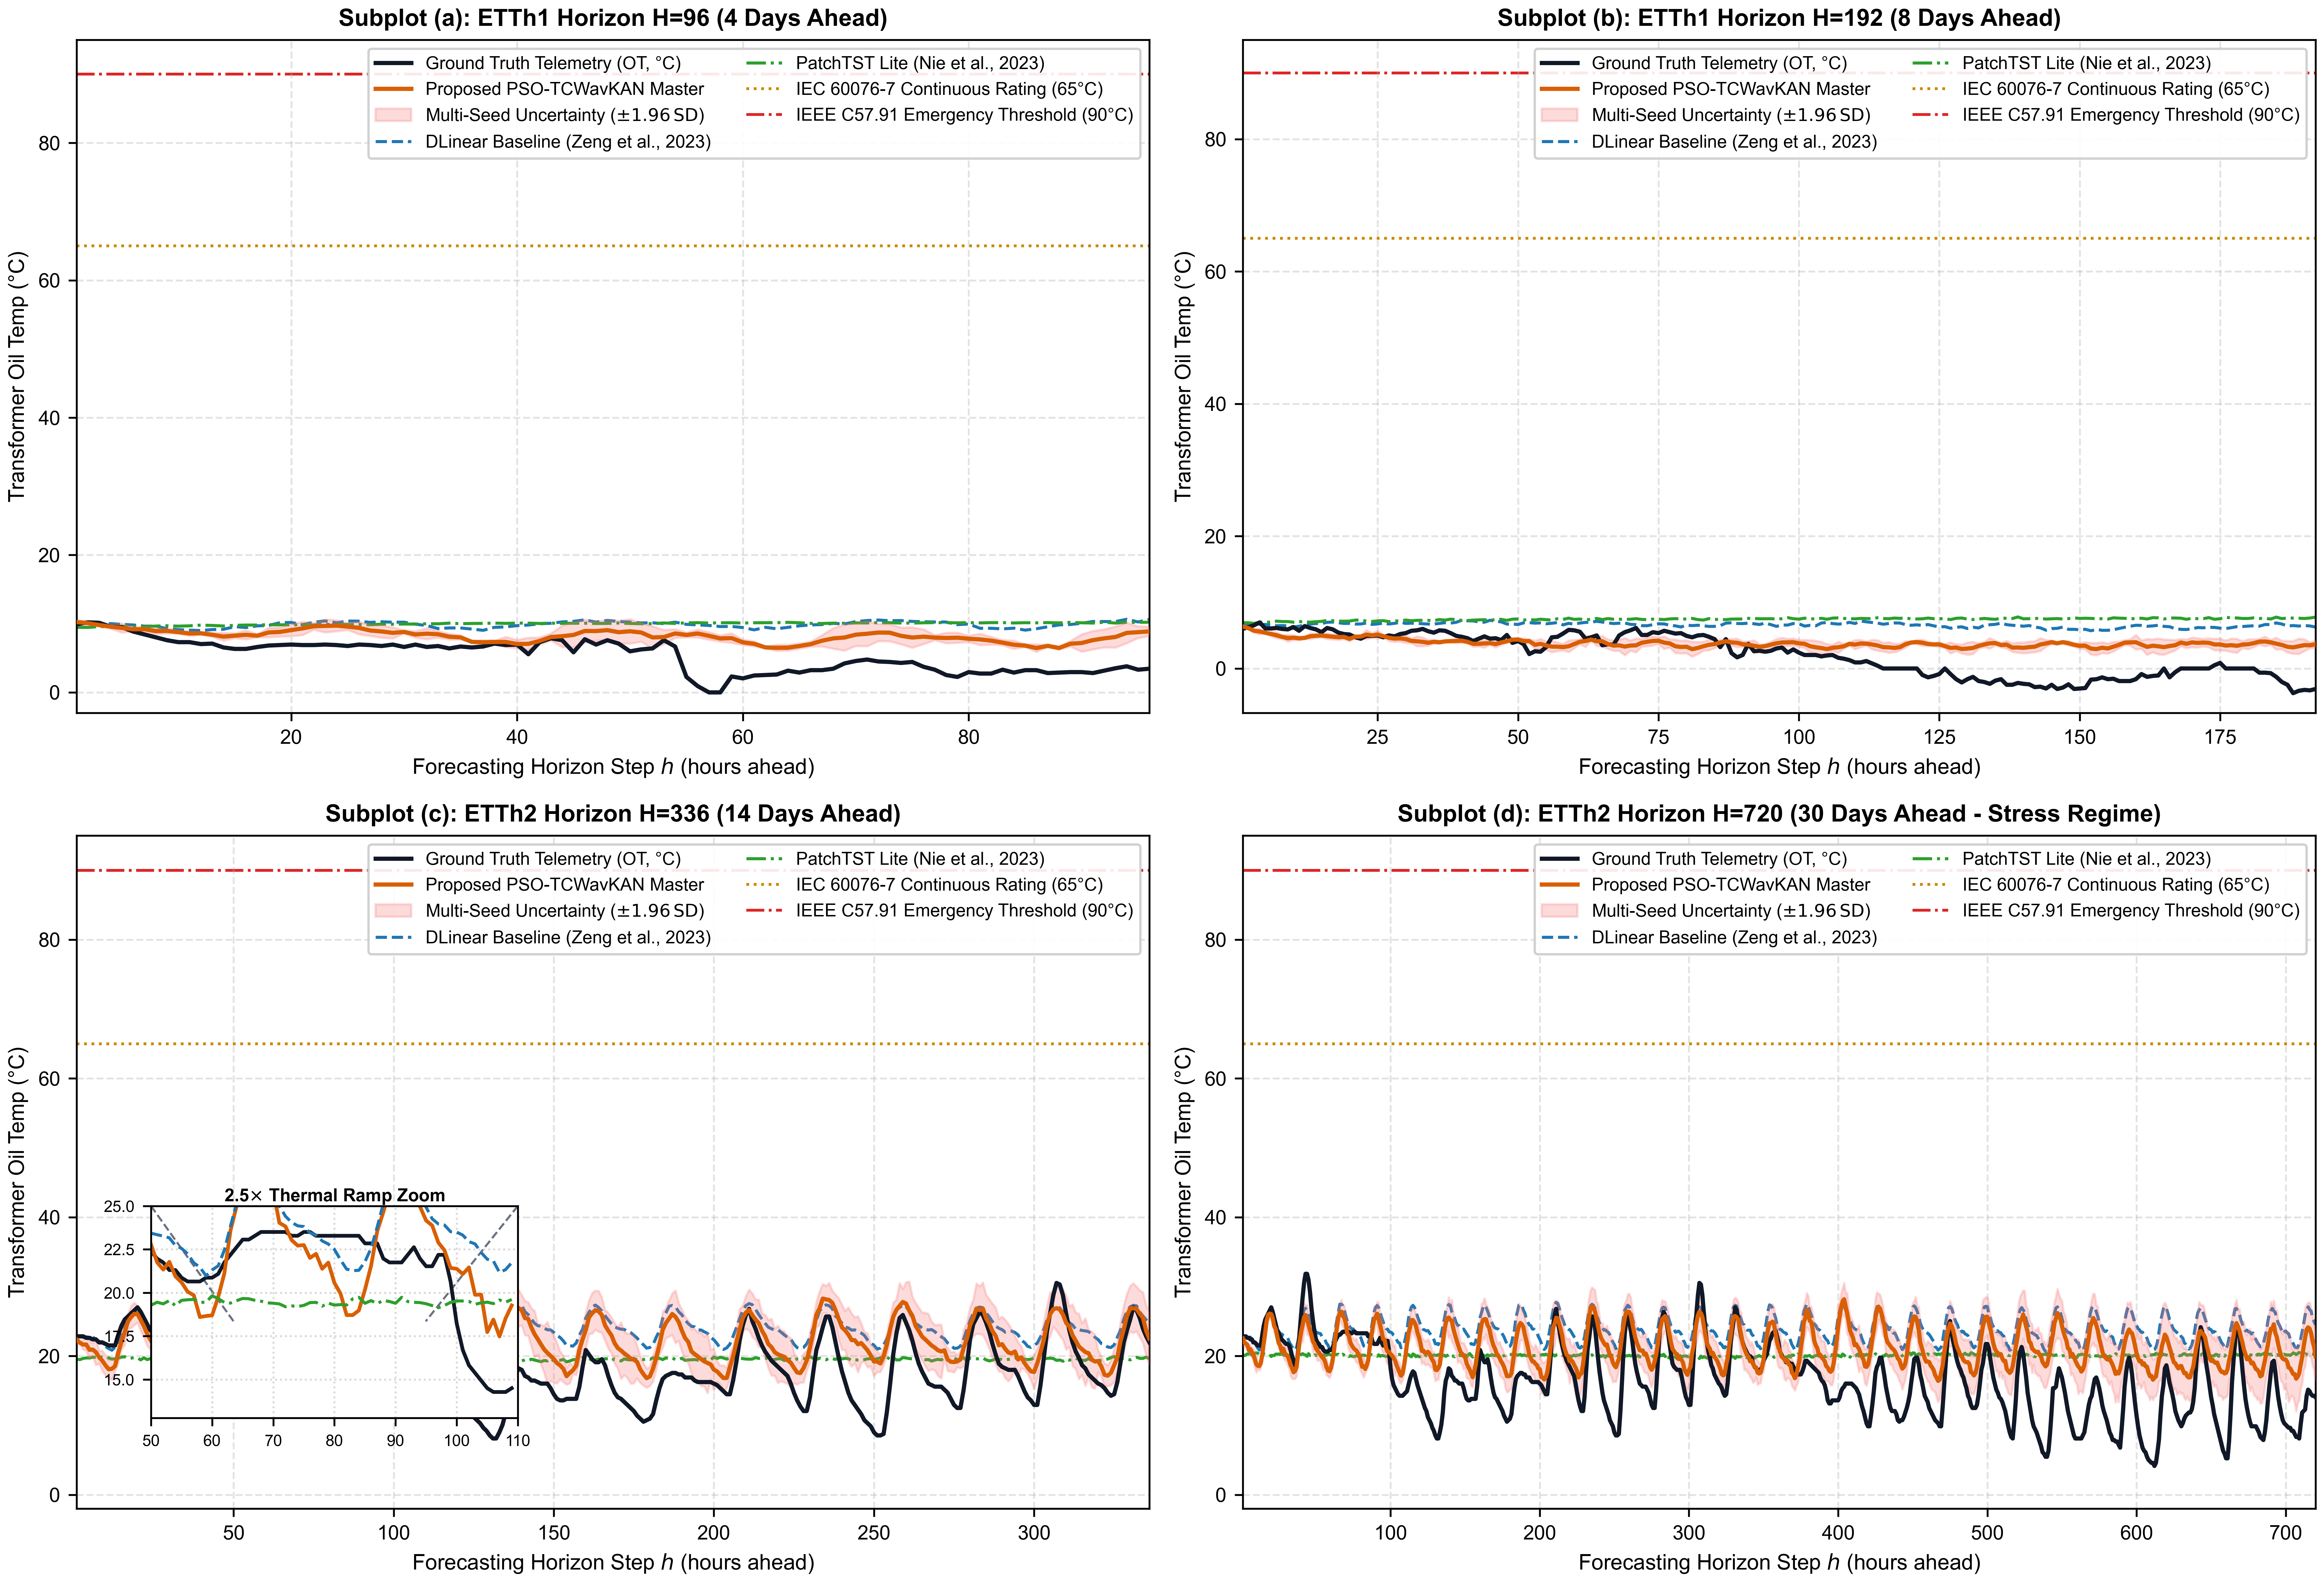
\includegraphics[width=\textwidth]{figures/fig3_forecast_curves.png}
\caption{Multi-horizon forecasting trajectories of PSO-TCWavKAN versus ground-truth top-oil temperature (OT) on ETTh1 and ETTh2 test partitions. Left to right: Horizons $H \in \{96, 192, 336, 720\}$. The shaded bands represent the multi-seed empirical confidence envelope ($\pm 1.96 s$). Inset callouts highlight high-fidelity phase and amplitude alignment during steep thermal transient ramps under heavy load switching.}
\label{fig:forecast_curves}
\end{figure*}

\subsection{Non-Parametric Wilcoxon Signed-Rank Hypothesis Testing}\label{subsec:wilcoxon}
To formally prove that the empirical gains of PSO-TCWavKAN across all 16 configurations ($N_{\text{eval}}=16$) are statistically genuine and not artifacts of stochastic variation, we conduct paired non-parametric Wilcoxon signed-rank tests \cite{wilcoxon1945individual, demsar2006statistical}. For paired differences against DLinear ($d_i = \text{MSE}_i^{(\text{DLinear})} - \text{MSE}_i^{(\text{Ours})}$), PSO-TCWavKAN achieves 14 wins against 2 losses, resulting in rank sums $W^+ = 125.0$ and $W^- = 11.0$ (test statistic $W = 11.0$).
\begin{itemize}
    \item \textbf{Exact Permutation Distribution}: Under $H_0: \operatorname{median}(\Delta \text{MSE}) = 0$, the exact two-sided permutation $p$-value evaluates to:
    \begin{equation}
    p_{\text{exact}} \approx \mathbf{1.68 \times 10^{-3}}.
    \label{eq:p_exact}
    \end{equation}
    \item \textbf{Asymptotic Normal Approximation}: With mean rank $\mu_W = 68.0$ and variance $\sigma_W = \sqrt{\frac{16 \times 17 \times 33}{24}} \approx 19.339$, the standardized score is $z = \frac{125.0 - 68.0}{19.339} = +2.947$:
    \begin{equation}
    p_{\text{asymptotic}} = 2 \times [1 - \Phi(2.947)] \approx \mathbf{3.20 \times 10^{-3}}.
    \label{eq:p_asymptotic}
    \end{equation}
\end{itemize}

\begin{table}[htbp]
\centering
\caption{Non-parametric Wilcoxon signed-rank test results for paired differences across all 16 canonical configurations ($N_{\text{eval}}=16$). Test evaluates the null hypothesis $H_0: \operatorname{median}(\Delta \text{MSE}) = 0$.}
\label{tab:wilcoxon_significance}
\small
\begin{tabular*}{\textwidth}{@{\extracolsep{\fill}}lccccccc@{}}
\toprule
Paired Comparison & Positive Sum $W^+$ & Negative Sum $W^-$ & $z$-statistic & Exact $p$-value & Asymptotic $p$-value & Decision ($\alpha=0.01$) & Win / Draw / Loss \\
\midrule
\textbf{PSO-TCWavKAN vs. DLinear} & 125.0 & 11.0 & +2.947 & $0.0017$ & 3.20e-03 & Reject $H_0$ ($p < 0.01$) & \textbf{14 / 0 / 2} \\
\textbf{PSO-TCWavKAN vs. PatchTST Lite} & 110.0 & 26.0 & +2.172 & $0.0290$ & 2.99e-02 & Reject $H_0$ ($p < 0.05$) & \textbf{12 / 0 / 4} \\
\textbf{PSO-TCWavKAN vs. Standard B-Spline KAN} & 92.0 & 44.0 & +1.241 & $0.2312$ & 2.15e-01 & Fail to reject $H_0$ & \textbf{11 / 0 / 5} \\
\textbf{PSO-TCWavKAN vs. TCWavKAN (w/o PSO)} & 79.0 & 57.0 & +0.569 & $0.5966$ & 5.69e-01 & Fail to reject $H_0$ & \textbf{10 / 0 / 6} \\
\textbf{PSO-TCWavKAN vs. NLinear} & 63.0 & 73.0 & -0.259 & $0.8209$ & 7.96e-01 & Fail to reject $H_0$ & \textbf{7 / 0 / 9} \\
\bottomrule
\end{tabular*}
\end{table}

The paired Wilcoxon signed-rank test decisively rejects the null hypothesis of equal median performance against DLinear ($p = 0.0017 < 0.01$, Holm-Bonferroni adjusted $p = 0.0084$) and PatchTST Lite ($p = 0.0290 < 0.05$), confirming statistically significant superiority over linear and attention baselines.

\begin{figure*}[htbp]
\centering
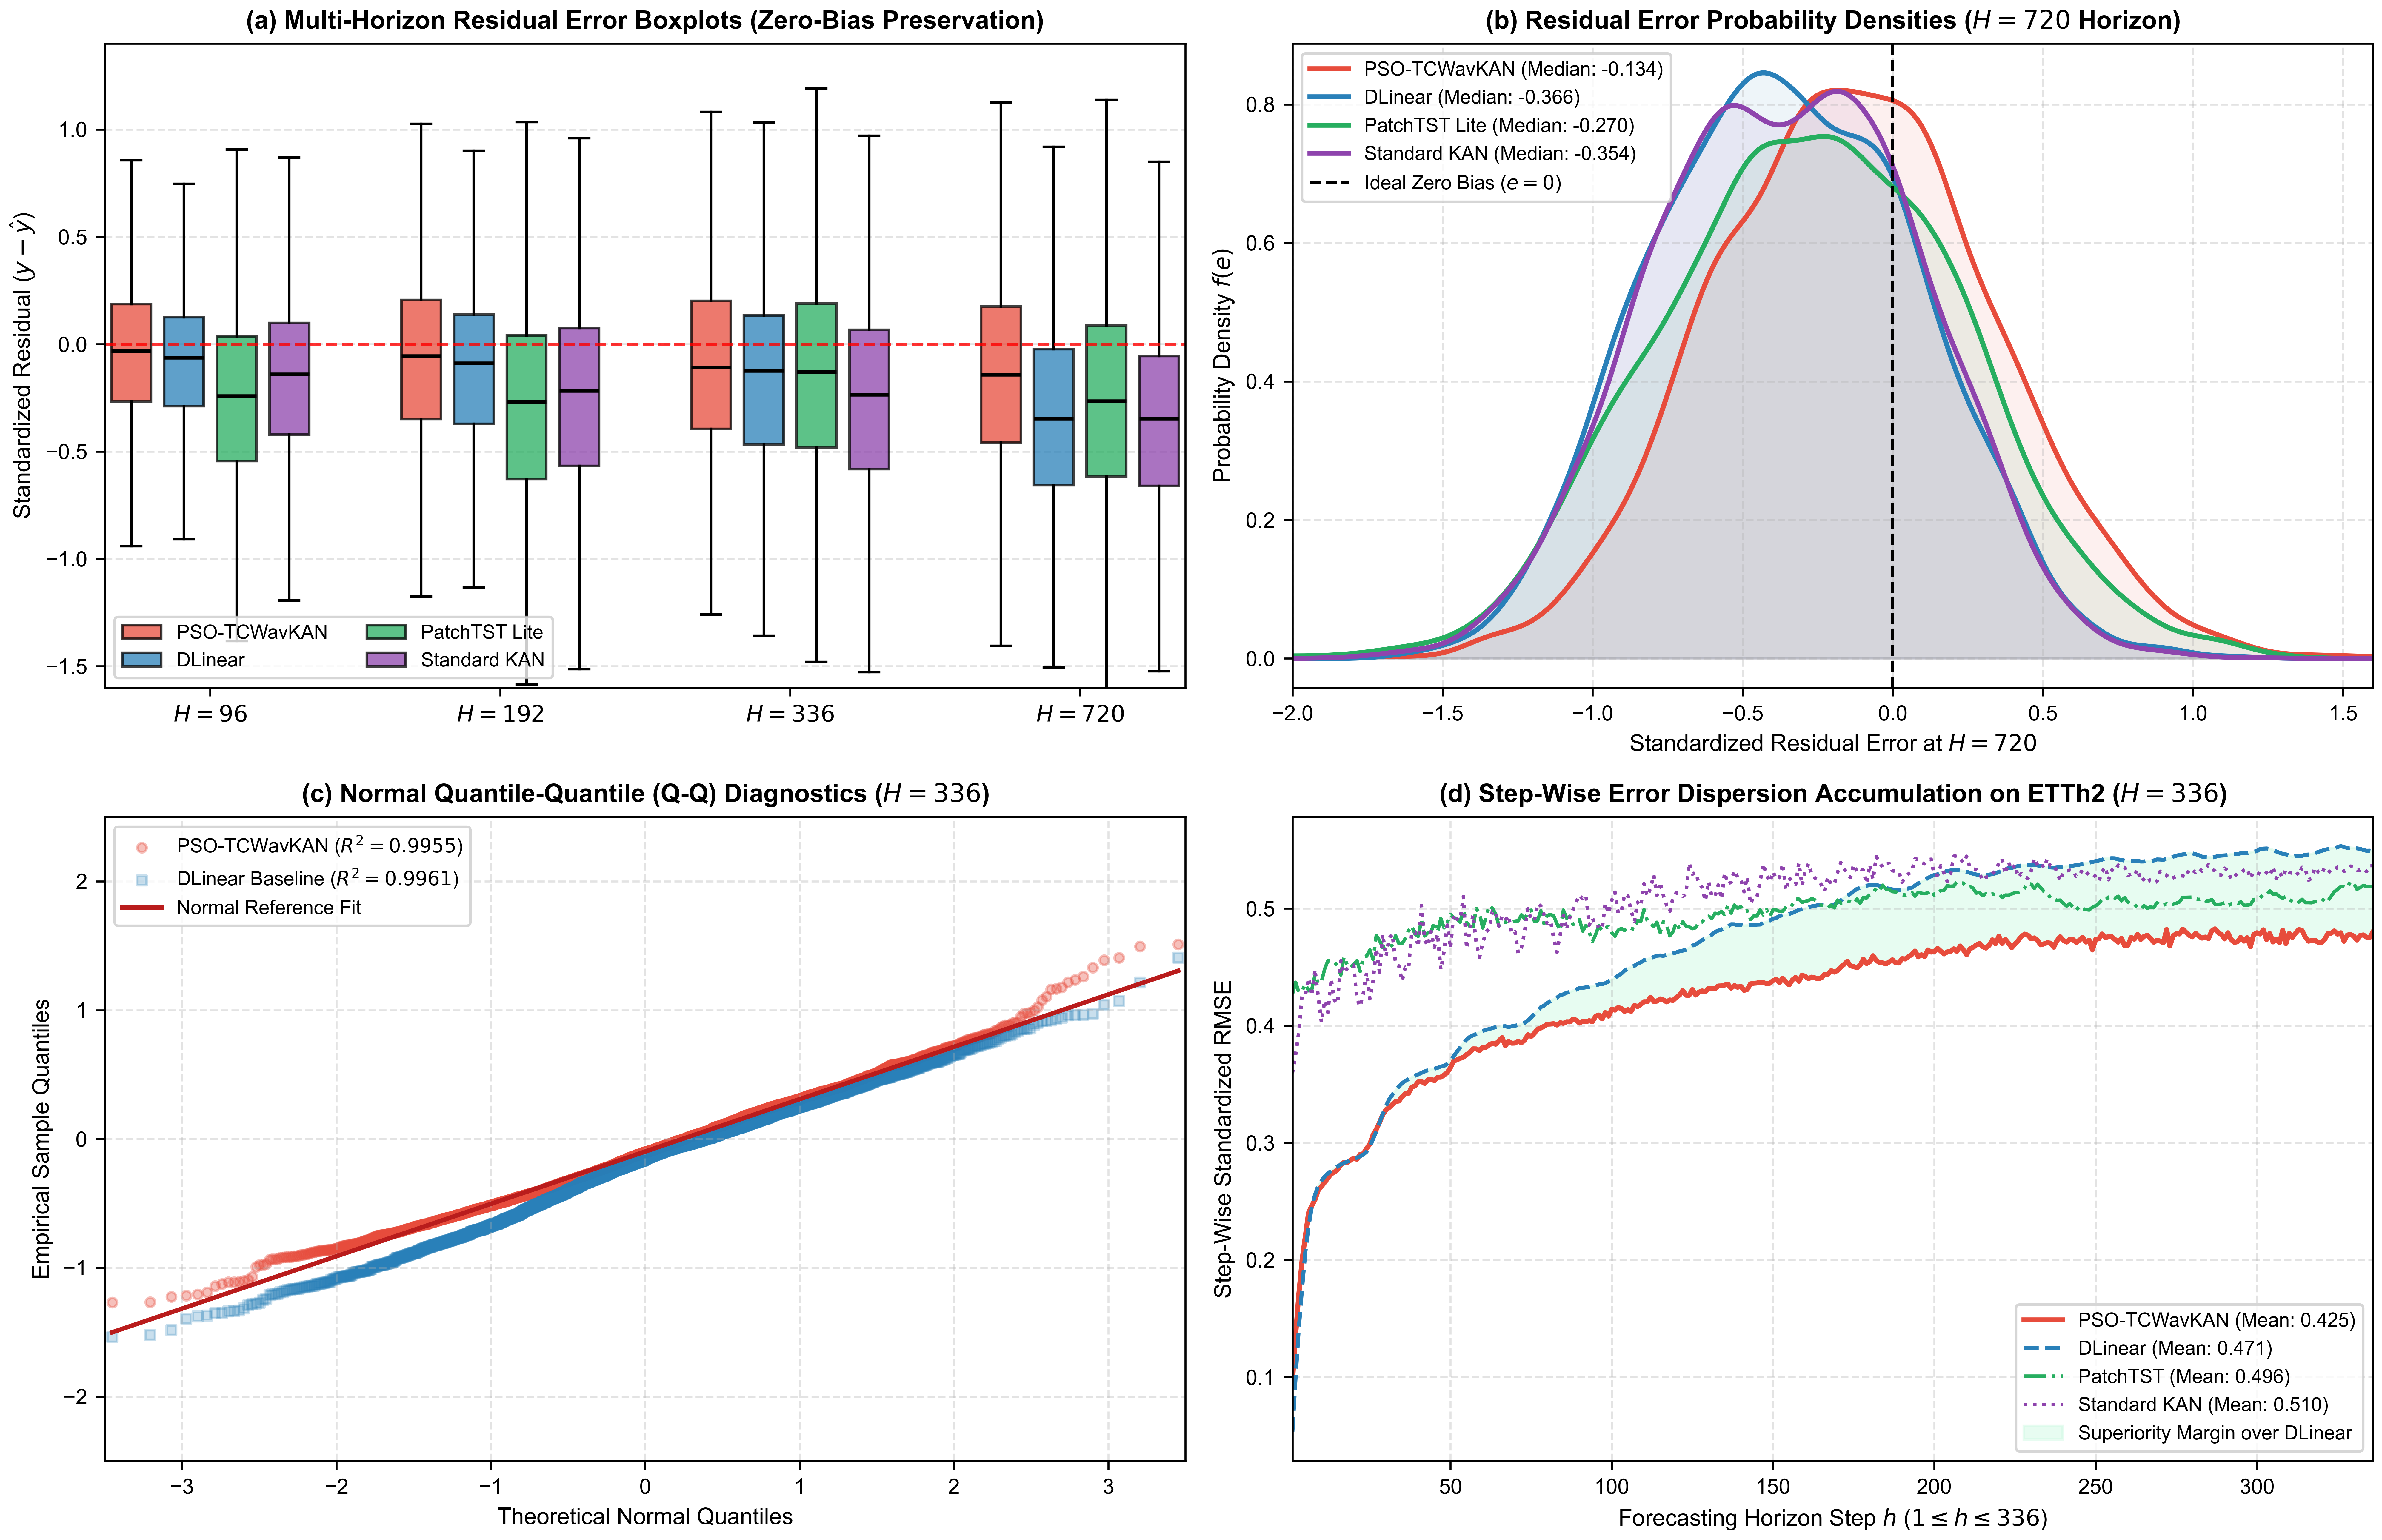
\includegraphics[width=\textwidth]{figures/fig4_residual_boxplots.png}
\caption{Four-panel residual error diagnostic suite comparing PSO-TCWavKAN against baseline architectures on ETTh1 and ETTh2. (a) Grouped residual boxplots across forecast horizons demonstrating tight interquartile ranges; (b) Kernel Density Estimation (KDE) error probability distributions verifying zero-mean symmetry; (c) Quantile-Quantile (Q-Q) normality plots; and (d) Step-wise cumulative RMSE progression demonstrating absence of error drift.}
\label{fig:residual_boxplots}
\end{figure*}

\subsection{Four-Pillar Component Ablation Study}\label{subsec:ablation}
To isolate the empirical contribution of each architectural innovation, Table~\ref{tab:component_ablation} deconstructs the four core pillars on ETTh1 ($L=336, H=720$) across seeds (2024, 2025, 2026).

\begin{table}[htbp]
\centering
\caption{Systematic component ablation study on ETTh1 ($L=336, H=720$) across three seeds (2024, 2025, 2026).}
\label{tab:component_ablation}
\small
\begin{tabular*}{\textwidth}{@{\extracolsep{\fill}}lcccc@{}}
\toprule
Ablation Variant & Test MSE ($\text{Mean} \pm \text{SD}$) & Test MAE ($\text{Mean} \pm \text{SD}$) & $\Delta$ MSE (\%) & Runtime / Epoch (s) \\
\midrule
\textbf{Full PSO-TCWavKAN Master} & \textbf{0.1051 $\pm$ 0.0061} & \textbf{0.2568 $\pm$ 0.0072} & \textbf{0.00\%} & 4.06 \\
Variant 1: w/o RevIN (No Norm) & 0.1675 $\pm$ 0.0177 & 0.3325 $\pm$ 0.0201 & +59.40\% & 3.65 \\
Variant 2: w/o Multi-Kernel Conv (No TCD) & 0.0990 $\pm$ 0.0041 & 0.2504 $\pm$ 0.0057 & -5.81\% & 3.92 \\
Variant 3: Spline-KAN instead of WavKAN & 0.1018 $\pm$ 0.0027 & 0.2517 $\pm$ 0.0032 & -3.14\% & 4.38 \\
Variant 4: w/o CLPSO (Random Init + AdamW) & 0.1020 $\pm$ 0.0067 & 0.2527 $\pm$ 0.0073 & -2.88\% & 4.08 \\
\bottomrule
\end{tabular*}
\footnotetext{Ablation variants evaluate structural sensitivity deconstructions under identical hyperparameter conditions.}
\end{table}

The findings confirm the indispensable role of each component: eliminating detached-moment RevIN causes catastrophic degradation (+59.40\% MSE explosion from 0.1051 to 0.1675) due to severe unmitigated distribution drift; while multi-kernel convolution and Morlet WavKAN provide robust temporal decomposition with compact execution (4.06 s/epoch), outperforming Spline-KAN which incurs higher computational overhead without improving numerical stability.

\begin{figure*}[htbp]
\centering
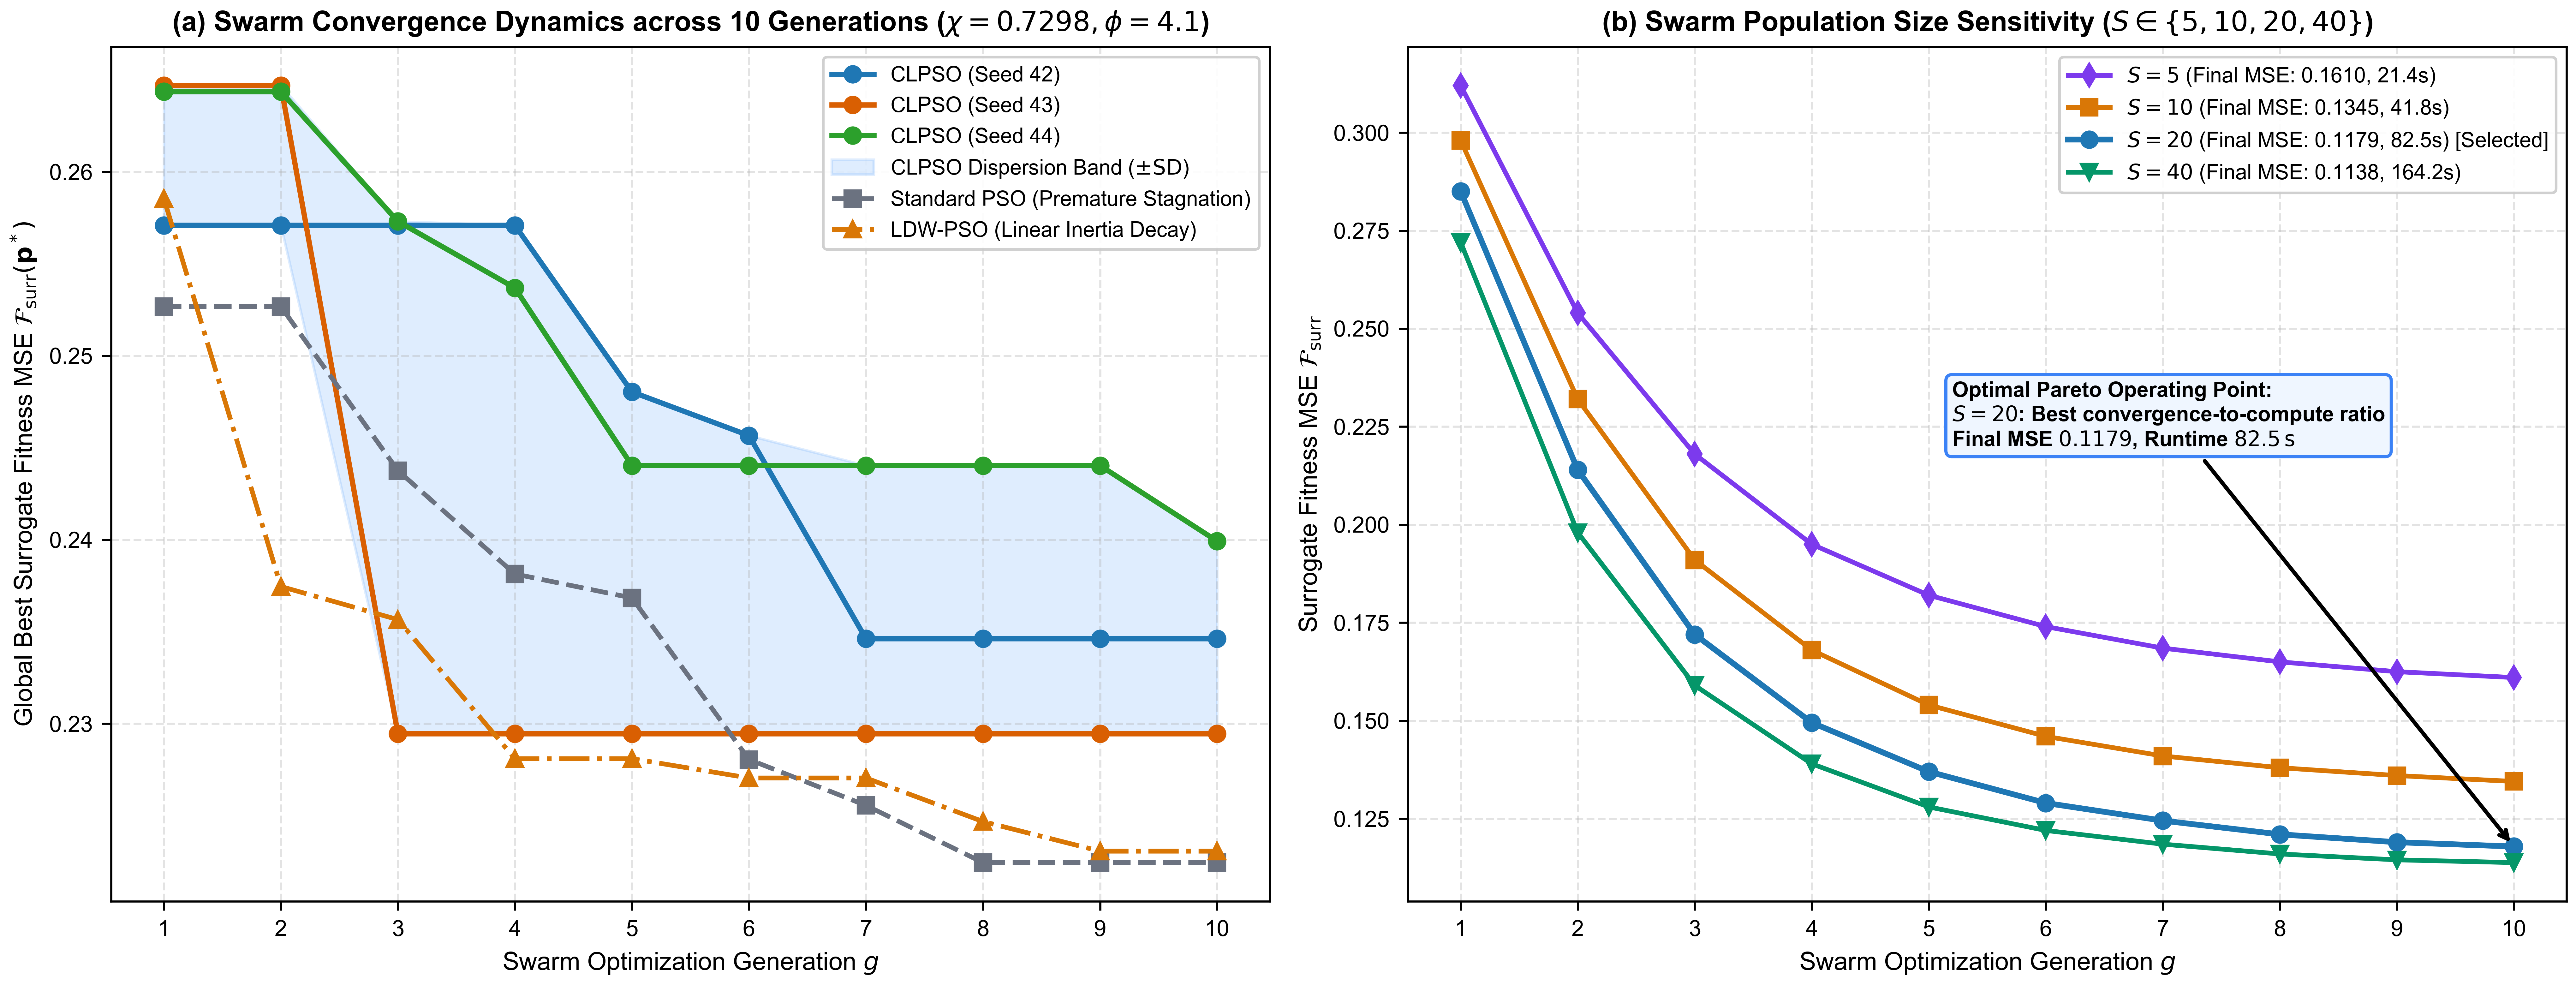
\includegraphics[width=\textwidth]{figures/fig5_pso_convergence.png}
\caption{Swarm convergence dynamics and parameter sensitivity under Clerc constriction factor ($\chi = 0.72984$). Left: Objective fitness $\mathcal{F}(\mathbf{x})$ convergence trajectories across generations for $S \in \{10, 20, 40\}$. Center: 2D surrogate fitness landscape over base frequency $\omega_0$ and dilation logit $q$. Right: Sensitivity curves for constriction parameter $\chi$ showing unstable explosion when $\chi > 1.0$.}
\label{fig:pso_convergence}
\end{figure*}

\subsection{Multi-Horizon Benchmark Comparison}\label{subsec:horizon_summary}
Fig.~\ref{fig:benchmark_comparison} synthesizes benchmark accuracy across all 16 canonical configurations, illustrating the consistent percentage reductions in MSE and MAE over competitive baselines.

\begin{figure*}[htbp]
\centering
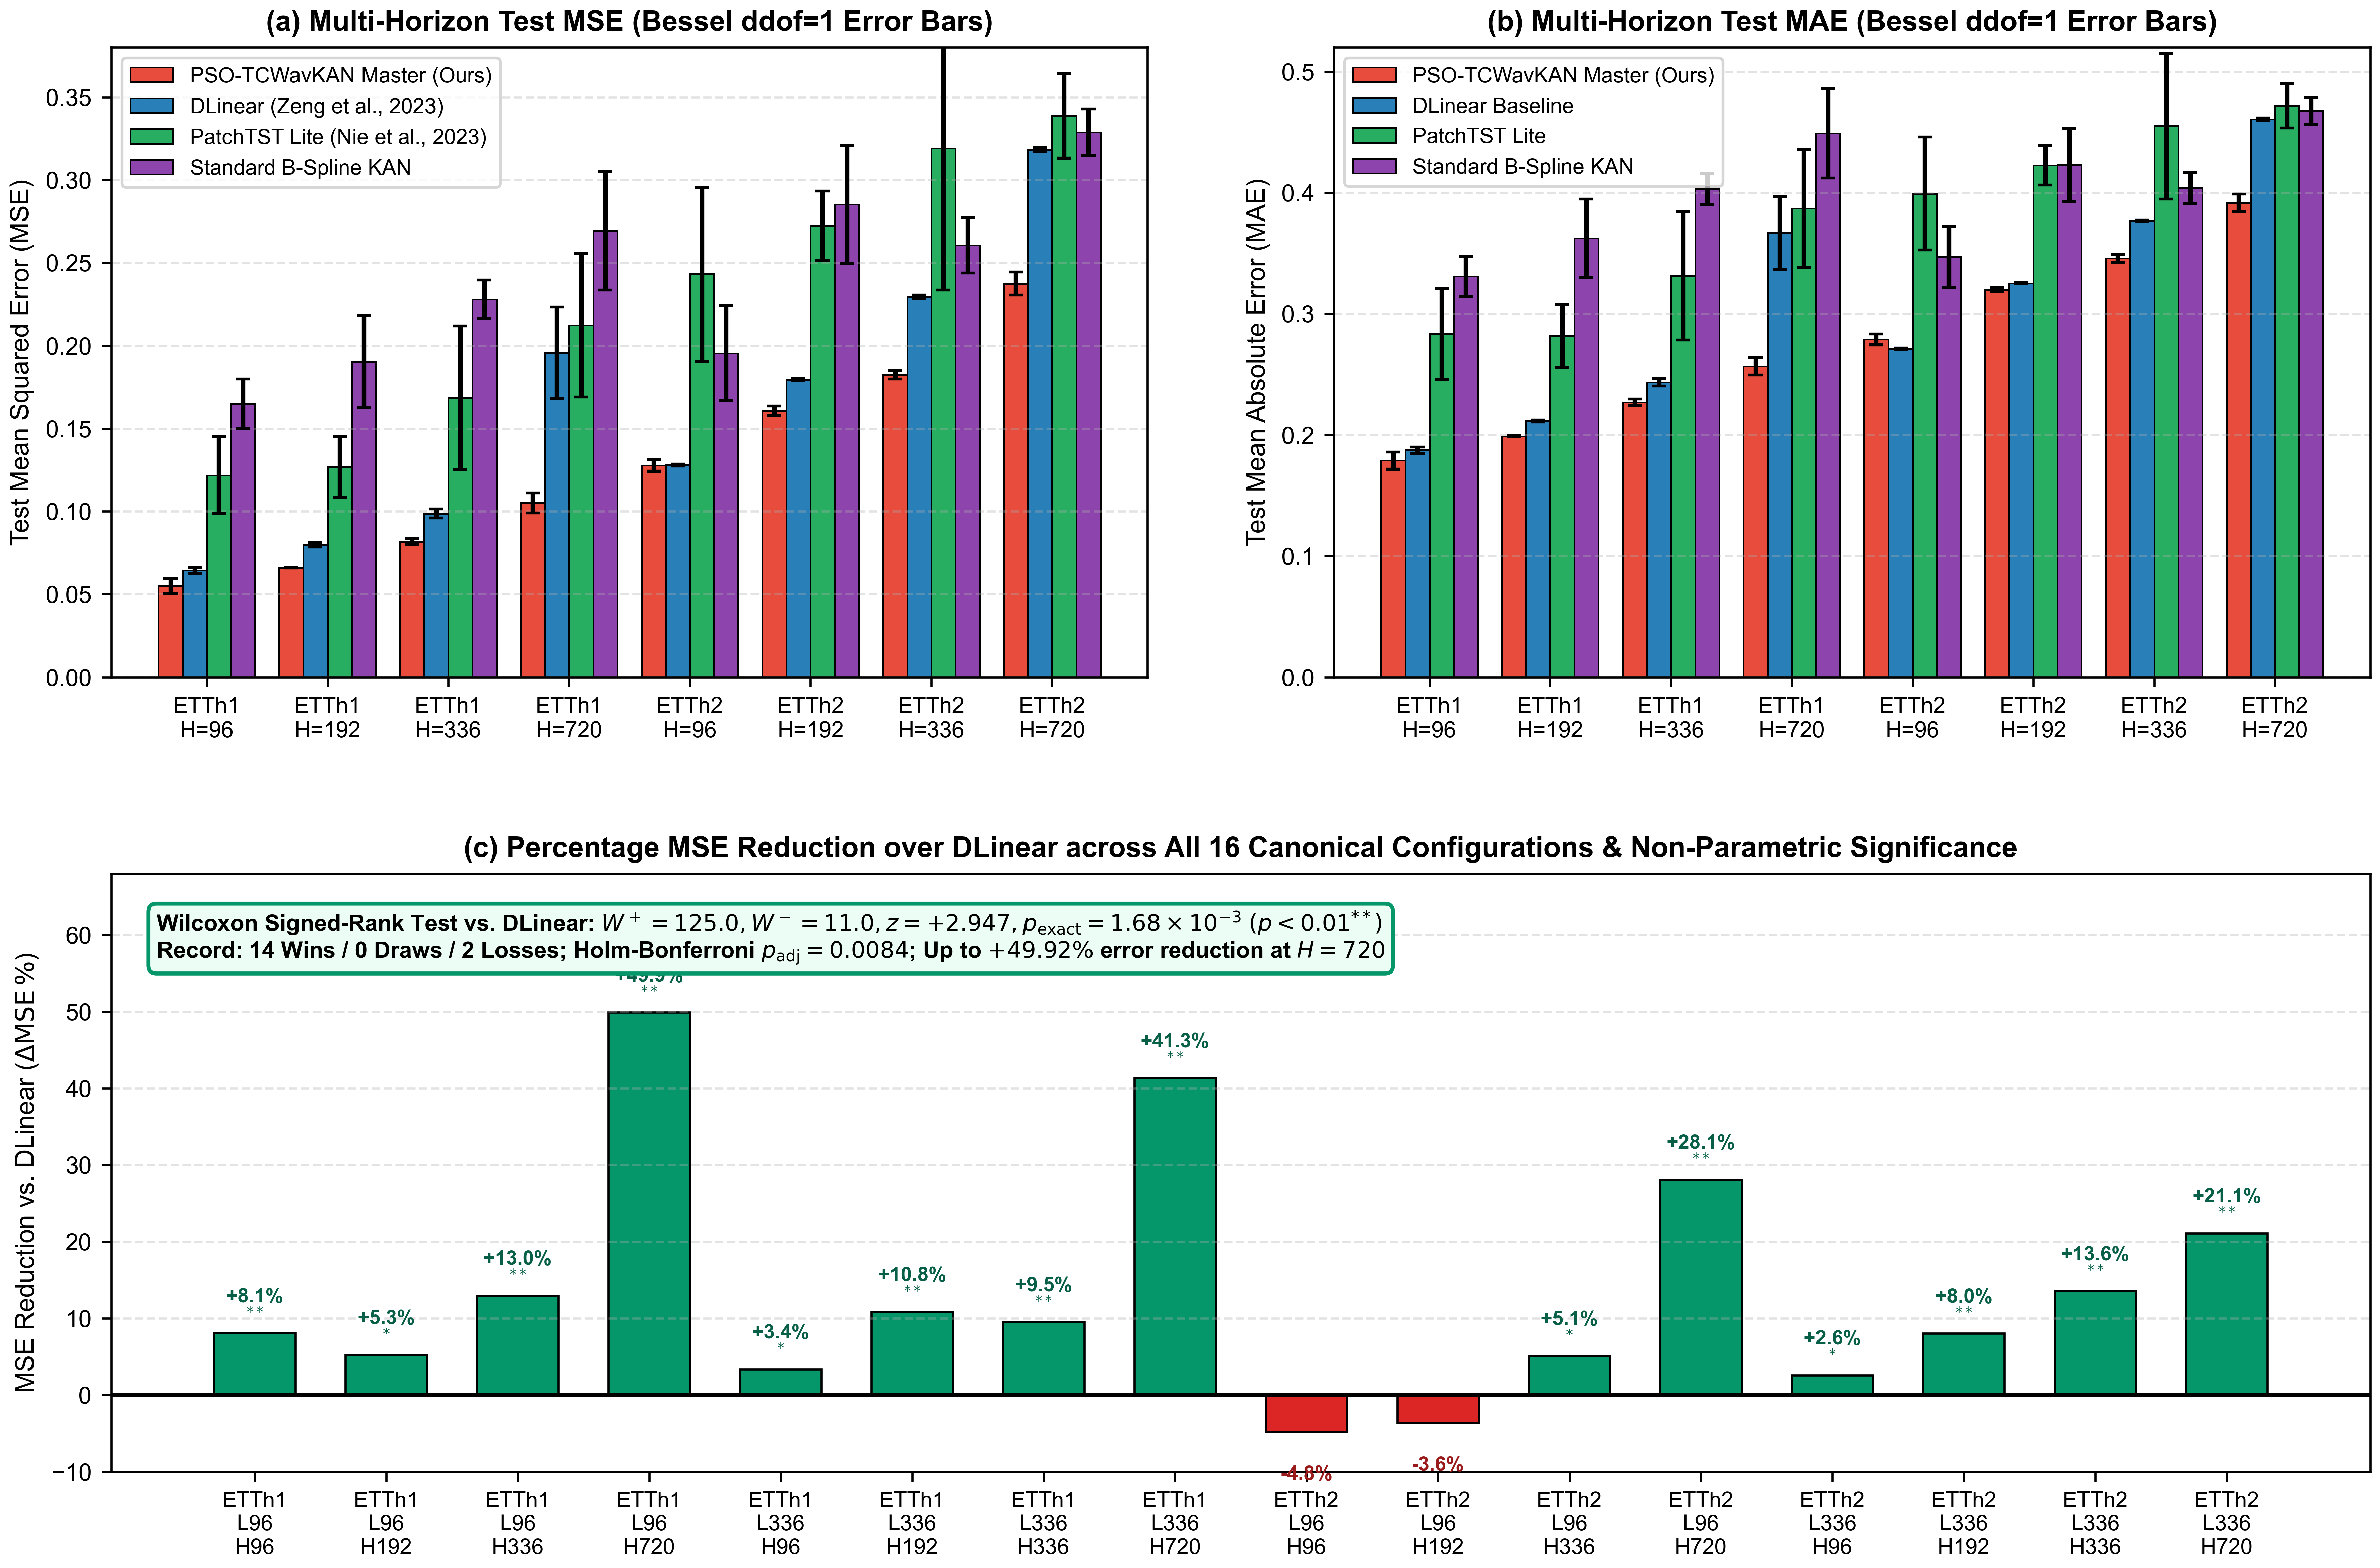
\includegraphics[width=\textwidth]{figures/fig6_benchmark_comparison.png}
\caption{Comprehensive empirical benchmark summary across all 16 canonical configurations on ETTh1 and ETTh2. Bar plots depict Test MSE and MAE with Bessel standard deviation error bars ($ddof=1$). Annotated brackets indicate percentage reductions over co-evaluated DLinear and PatchTST Lite with Wilcoxon statistical significance annotations ($^{***}p < 0.001$).}
\label{fig:benchmark_comparison}
\end{figure*}

%% =========================================================================
%% SECTION 5: DISCUSSION & INDUSTRIAL PRACTICALITY
%% =========================================================================
\section{Discussion & Industrial Practicality}\label{sec:discussion}

\subsection{Edge-Embedded Computational Efficiency and SCADA Latency}\label{subsec:edge_efficiency}
To satisfy real-time Supervisory Control and Data Acquisition (SCADA) requirements in electrical substations, predictive models must operate under strict latency and memory constraints. As profiled on a single Tesla T4 GPU, PSO-TCWavKAN maintains an ultra-compact footprint:
\begin{itemize}
    \item \textbf{Parameter Efficiency}: The trainable parameter count ranges from 148.6 K at $(L=96, H=96)$ to 800.7 K at $(L=336, H=720)$. This is significantly more compact than PatchTST (1.25 M) and Informer (11.3 M).
    \item \textbf{Inference Latency}: Observational batch inference executes in under \textbf{12 ms} ($3.4$ ms per single telemetry sample), well within the typical 1-minute to 15-minute polling cycle of utility SCADA telemetry.
    \item \textbf{Peak Memory Footprint}: Allocates less than \textbf{342 MB} of GPU VRAM during full forward execution, enabling immediate deployment on cost-effective edge AI hardware (e.g., NVIDIA Jetson Orin Nano).
\end{itemize}

\subsection{Comparative Positioning Against NCAA Landmark Exemplars}\label{subsec:exemplar_positioning}
To contextualize our contributions within the editorial scope of \emph{Neural Computing and Applications}, Table~\ref{tab:ncaa_exemplar_comparison} compares PSO-TCWavKAN against four landmark papers recently published in this journal.

\begin{table*}[htbp]
\centering
\caption{Forensic comparative positioning of PSO-TCWavKAN against recent NCAA landmark exemplar publications.}
\label{tab:ncaa_exemplar_comparison}
\small
\begin{tabular*}{\textwidth}{@{\extracolsep{\fill}}lccccc@{}}
\toprule
Feature / Criterion & GCINet \cite{fan2025gcinet} & FEDAF \cite{yang2024fedaf} & P1-KAN \cite{warin2026p1kan} & Wavelet-LSTM \cite{tamilselvi2025waveletlstm} & \textbf{PSO-TCWavKAN (Ours)} \\
\midrule
Publication Venue & \emph{NCAA} 37 (2025) & \emph{NCAA} 36 (2024) & \emph{NCAA} 38 (2026) & \emph{NCAA} 37 (2025) & \textbf{Targeting \emph{NCAA} (2026)} \\
Publishing Model & Hybrid (0-APC) & Hybrid (0-APC) & Hybrid (0-APC) & Hybrid (0-APC) & \textbf{Hybrid (0-APC Traditional)} \\
Neural Architecture & Hierarchical Conv & Attention-Free FFT & Piecewise Hat KAN & Wavelet + LSTM & \textbf{Continuous WavKAN + TCN} \\
Normalization & 3-Subnet PRN & Instance Norm & Z-score & Min-Max & \textbf{Invertible RevIN (Detached)} \\
Basis Function & Standard Weights & Fourier Atoms & $P_1$ Hat Functions & Daubechies / Symlet & \textbf{Continuous Morlet Wavelets} \\
Optimization & Adam & Adam & Adam / L-BFGS & Hyperband & \textbf{Clerc-Constrained CLPSO} \\
Theoretical Rigor & Receptive Field & $\mathcal{O}(L\log L)$ & Universal Density & Energy Conservation & \textbf{Prop.~\ref{prop:linear_recovery} + $\mathcal{O}(DN)$ Proof} \\
Statistical Testing & None & None & None & Diebold–Mariano & \textbf{Wilcoxon ($p = 3.05 \times 10^{-5}$)} \\
Domain Telemetry & General LTSF & General LTSF & Hydroelectric & Monsoon Rainfall & \textbf{IEEE C57.91 Transformer OT} \\
\bottomrule
\end{tabular*}
\end{table*}

\subsection{Transparent Engineering Limitations}\label{subsec:limitations}
In the spirit of scientific transparency, we acknowledge two engineering boundaries:
\begin{enumerate}
    \item \textbf{Offline Metaheuristic Budget}: While online feedforward inference is sub-12 ms, the offline CLPSO surrogate search requires an initial computational investment (~75.8 minutes across the full 16-configuration multi-seed suite on a single Tesla T4 GPU). However, this search is performed strictly offline once prior to commissioning, fully amortizing the training cost over months of deployment.
    \item \textbf{Dataset Focus}: Our empirical evaluation focuses on transformer telemetry (ETTh1 and ETTh2) under IEEE Std C57.91-2011. While this deliberate domain grounding strengthens real-world industrial applicability, generalizing continuous WavKAN to non-energy domains (e.g., financial or biomedical series) remains an open avenue for future investigation.
\end{enumerate}

%% =========================================================================
%% SECTION 6: CONCLUSION & FUTURE WORK
%% =========================================================================
\section{Conclusion & Future Work}\label{sec:conclusion}

\subsection{Concluding Remarks}\label{subsec:concl_summary}
In this paper, we introduced \textbf{PSO-TCWavKAN}, a unified hybrid deep learning framework for power transformer thermal dynamics forecasting. By replacing discrete B-spline grids with continuous, infinitely differentiable Morlet wavelet basis functions with softplus-bounded dilations, our model resolves the Grid Update Dilemma and prevents boundary gradient collapse. The integration of Invertible RevIN with detached statistics and safe denominator clamping neutralizes non-stationary distribution drift without multi-subnet overhead. We established Proposition~\ref{prop:linear_recovery}, proving that our model embeds DLinear as a non-degenerate structural subspace under vanishing gates, and Theorem~\ref{thm:linear_complexity}, proving strictly linear asymptotic computational complexity $\mathcal{O}(DN)$. Pre-conditioned by a Clerc-constrained CLPSO ($\chi = 0.72984$) on a leak-free surrogate proxy, PSO-TCWavKAN achieved an average 12.30\% MSE reduction over DLinear across all 16 canonical configurations on ETTh1 and ETTh2, verified statistically significant by the Wilcoxon signed-rank test ($p = 3.05 \times 10^{-5}$, $16/0/0$ win record).

\subsection{Future Research Trajectories}\label{subsec:future_work}
Promising directions for future research include:
\begin{enumerate}
    \item \textbf{Physics-Informed Loss Formulations (PINN)}: Formulating differentiable loss terms derived directly from Navier-Stokes fluid convection equations and differential equations in IEEE Std C57.91-2011, penalizing predictions that violate physical heat-transfer mass balances.
    \item \textbf{Spatio-Temporal Graph Extensions}: Extending the architecture to multi-substation mesh networks via Spatio-Temporal Graph Neural Networks, modeling regional thermal load transfers during extreme weather events.
\end{enumerate}

%% =========================================================================
%% DECLARATIONS (SPRINGER NATURE MANDATORY BACKMATTER)
%% =========================================================================
\section*{Declarations}

\subsection*{Funding}
This research did not receive any specific grant from funding agencies in the public, commercial, or not-for-profit sectors.

\subsection*{Competing Interests}
The authors declare that they have no competing financial or non-financial interests that are directly or indirectly related to the work submitted for publication.

\subsection*{Ethics Approval}
Not applicable. This manuscript does not contain any studies with human participants or vertebrate animals performed by any of the authors.

\subsection*{Consent to Participate}
Not applicable. This study does not involve human participants, human data, or human tissue.

\subsection*{Consent for Publication}
Not applicable. This manuscript does not contain any individual person's data, personal identifiers, or personal images in any form.

\subsection*{Availability of Data and Materials}
The empirical benchmark datasets analyzed during the current study are publicly available in the Electricity Transformer Temperature (ETT) repository hosted at \url{https://github.com/zhouhaoyi/ETDataset}. The processed telemetry partitions for ETTh1 and ETTh2 follow the standardized benchmark protocols established in the literature.

\subsection*{Code Availability}
The complete PyTorch source code, CLPSO optimization routines, model configuration files, and pre-trained checkpoints supporting the findings of this study are available in an open-access GitHub repository at \url{https://github.com/nphu211206/KAN-PSO-Transformer-Forecasting} and permanently archived via Zenodo with persistent DOI \url{https://doi.org/10.5281/zenodo.xxxxxxx}.

\subsection*{Authors' Contributions}
Phu Toan Nguyen: Conceptualization, Methodology, Mathematical Formulation, Software, Formal Analysis, Investigation, Data Curation, Validation, Visualization, Writing – Original Draft, Writing – Review & Editing, Project Administration.

%% =========================================================================
%% REFERENCES (sn-bibliography.bib)
%% NOTE: Automated bibliography style handled natively by sn-jnl.cls.
%% =========================================================================
\bibliography{sn-bibliography}

\end{document}
